\documentclass[12pt,a4paper,timesnewroman,twoside,openright]{report}

%\usepackage{polyglossia}
%\setdefaultlanguage{english}
%\setotherlanguage{hindi}
%\usepackage{fontspec}
%\newfontfamily\devanagarifont{}
%\usepackage[T1]{fontenc}
% \usepackage[backend=biber]{biblatex}
% \addbibresource{References.bib}
\usepackage{titlesec}
\titleformat
{\chapter} % command
[display] % shape
{\normalfont \bfseries \Huge \setstretch{1}} % format
{\itshape \chaptertitlename\  \thechapter} % label
{0.5ex} % sep
{
	%\rule{\textwidth}{1pt}
	\vspace{2.5ex}
	%\centering
} % before-code
[
\vspace{-1ex}%
%\rule{\textwidth}{0.3pt}
] % after-code


\titleformat{\section}[hang]{\normalfont \LARGE \bfseries \setstretch{1}}{\thesection.}{0.5em}{}

\titlespacing{\section}{0.5ex}{5ex}{-0.5ex}

\titleformat{\subsection}[hang]{\normalfont \large \bfseries \setstretch{1}}{\thesubsection.}{0.5em}{}

\titlespacing{\subsection}{0.9ex}{5ex}{-0.5ex}

\titleformat{\subsubsection}[hang]{\normalfont \normalsize \bfseries \setstretch{1}}{\thesubsubsection.}{0.5em}{}

\titlespacing{\subsubsection}{1.3ex}{5ex}{-0.5ex}

\newcommand{\changelocaltocdepth}[1]{%
	\addtocontents{toc}{\protect\setcounter{tocdepth}{#1}}%
	\setcounter{tocdepth}{#1}%
}
\usepackage{longtable}
\usepackage{caption}
\DeclareCaptionFont{mysize}{\fontsize{11}{15}\selectfont}
\captionsetup{font=mysize}
\usepackage{booktabs}% http://ctan.org/pkg/booktabs
\newcommand{\tabitem}{~~\llap{\textbullet}~~}
\usepackage{amsmath,amsfonts}
\usepackage{lscape}
\usepackage{cite}
\usepackage{afterpage}
\newcommand\blankpage{%
    \null
    \thispagestyle{empty}%
    \addtocounter{page}{-1}%
    \newpage}

\usepackage{setspace}	% for line spacing
\usepackage{graphicx,subfig,tikz}
\usetikzlibrary{arrows}
\usepackage{pdflscape}
\usepackage{tcolorbox}
%\usepackage{epstopdf}
\usepackage{multirow}
\usepackage{paralist}
\usepackage{float}
\usepackage{secdot}
\setcounter{tocdepth}{2}
\setcounter{secnumdepth}{3}
\usepackage{enumitem}

\newcommand{\frontSign}[2]{%
    \begin{minipage}[t]{.3\textwidth}
        \centering
        \dotfill\\
        #1\\
        #2
    \end{minipage}%
    }
\usepackage{rotating}
\usepackage [autostyle, english = british]{csquotes}
\MakeOuterQuote{"}

\usepackage{titlesec}

\titleformat{\chapter}[display]
  {\filleft\bfseries\large}
  {\itshape\chaptername\ \thechapter}
  {-1em}
  {\bfseries\Huge}
\titlespacing*{\chapter}
  {0pt}
  {-1em}
  {1pt}

  
\usepackage{pdfpages}
% \usepackage[margin=1in]{geometry}
% \usepackage{lipsum}
% \newcommand\signature[3]{% Name; Department
% \noindent\begin{minipage}{4cm}
%     \noindent\vspace{3cm}\par
%     \noindent\rule{4cm}{1pt}\par
%     % \noindent\textbf{#1}\par
%     % \noindent#2%
% \end{minipage}}
% \newcommand\insertdate[1][\today]{\vfill\begin{flushright}#1\end{flushright}}

\usepackage{algorithm}
\usepackage[noend]{algpseudocode}
\usepackage[labelfont=bf]{caption}
\usepackage[title,toc,page]{appendix}
\usepackage{emptypage}

\usepackage{IEEEtrantools}
\usepackage[top=25mm, bottom=25mm, right=25mm, left=38mm]{geometry}
\usepackage{color}
\definecolor{nithred}{rgb}{0.5,0,0}
\definecolor{nithblue}{rgb}{0,0,0.5}
\definecolor{nithdarkred}{rgb}{0.2,0,0}
\definecolor{nithdarkblue}{rgb}{0,0,0.2}
\definecolor{nithgreen}{rgb}{0,0.2,0}
\usepackage[intoc]{nomencl}
\makenomenclature
%% This rename the main title:
\renewcommand{\nomname}{List of Abbreviations and Symbols}
%% this modifies item separation:
\setlength{\nomitemsep}{8pt}
%% this part defines the groups:
%----------------------------------------------
\RequirePackage{ifthen}
\renewcommand{\nomgroup}[1]{%
	\ifthenelse{\equal{#1}{A}}{\item[\Large\textbf{List of Abbreviations}]}
	\newpage {%
		\ifthenelse{\equal{#1}{S}}{\hspace{2cm}\item[\Large\textbf{List of Symbols}]}{}}}
		
%----------------------------------------------
% this line must be used in built command if using texstudio otherwise in terminal
%makeindex report.nlo -s nomencl.ist -o report.nls

%% for watermark %%
\usepackage{eso-pic}
\newcommand\BackgroundPic{
	\put(13,0){
		\parbox[b][\paperheight]{\paperwidth}{%
			\vfill
			\centering
			
\includegraphics[width=0.6\paperwidth,height=0.6\paperheight,
			keepaspectratio]{Initial_Pages/logo/nithwatermark.jpg}%
			\vfill
}}}

%%% Add this %%%
%\usepackage{titlesec}
%\titleformat{\chapter}[display]
%{\normalfont\huge\bfseries}{\chaptertitlename~\thechapter}{20pt}{\Huge}
%\titlespacing*{\chapter}{0pt}{50pt}{40pt}
%\titlespacing*{name=\chapter,numberless}{0pt}{-30pt}{10pt}
%%%   End   %%%
%%%%%%%%%%%%
\newcommand{\insertchapterspace}{%
	\addtocontents{lof}{\protect\addvspace{10pt}}%
	\addtocontents{lot}{\protect\addvspace{10pt}}%
}

% fancy header
%%\usepackage{fancyhdr}
%\fancyhead[RE]{\bf \nouppercase{\rightmark}}
%\fancyhead[LO]{\bf \nouppercase{\leftmark}}
%\fancyhead[RO]{\thepage}
%\fancyhead[LE]{\thepage}
%\fancyfoot{}
%\renewcommand{\headrulewidth}{0pt}
%\renewcommand{\footrulewidth}{0pt}
\newtheorem{lemma}{Lemma}
\newtheorem{theorem}{Theorem}
\newtheorem{corollary}{Corollary}

\newcommand{\figurewidth}{0.85\textwidth}
\newcommand{\figureheight}{0.35\textheight}

\DeclareRobustCommand{\ig}{\lowercase{ig}}
\DeclareRobustCommand{\IG}{\uppercase{IG}}
\usepackage{titletoc}
\titlecontents{chapter}
[0pt]% <left>
{\bfseries}% <above-code>
{\chaptername\ \thecontentslabel:\quad}% <numbered-entry-format>
{}% <numberless-entry-format>
{\titlerule*[0.8pc]{.}\contentspage}
%\usepackage{tocloft}
%\renewcommand{\cftfigfont}{Figure }
%\renewcommand{\cfttabfont}{Table }
%\titleformat{\chapter}[display]
%{\normalfont\huge \bfseries}{\chaptertitlename\ \thechapter}{5pt}{\Huge}
%{\normalfont \huge \filleft \bfseries\color{black}}{\chaptertitlename\ \thechapter}{8pt}{\LARGE}
%\titlespacing*{\chapter}{0pt}{0pt}{0pt}
%\graphicspath{{./Figures/}}
%\renewcommand\cftaftertoctitle{\par\noindent\rule{\textwidth}{2pt}\par\vskip-3.5em}
%\renewcommand\cftafterloftitle{\par\noindent\rule{\textwidth}{2pt}\par\vskip-3.0em}
%\renewcommand\cftafterlottitle{\par\noindent\rule{\textwidth}{2pt}\par\vskip-3.0em}
%\renewcommand\refname{\par\noindent\rule{\textwidth}{2pt}\par\vskip-3.0em}
%\usepackage[colorlinks=true,citecolor=black,linkcolor=black]{hyperref}
\begin{document}
	
	\pagestyle{empty}
	\include{Initial_Pages/coverpage}
	~
\vspace{8cm}
\begin{center}
$\qquad $ 
\end{center}
\vfill
~
	
	\begin{titlepage}
\begin{center}

%\textsc{}\\[0.5cm]



{\Large \textbf{Ocular Disease Classification using OCT Scans and Deep Learning: CNN and Autoencoders}}\\[1.0cm]

\textsc{\large \textbf{A Dissertation}}\\

{ \textit{Submitted in fulfillment of the requirements for the award of the degree of}}\\[1.0cm]

{\large \textbf{Master of Technology (Dual Degree)}}\\[0.5cm]

{ \textit{in}}\\[0.5cm]

{\large \textbf{ Electronics and Communication Engineering}}\\[1.0cm]

%\large in \\[.5cm]
{\large \textbf{\textit{Submitted by}}}\\[0.5cm]

{\large \textbf{Aniket Srivastava}}\\
{\large \textbf{(Roll No.: 184555)}}\\[1.0cm]

{\large \textbf{\textit{Under the supervision of}}}\\[0.25cm]
{\large \textbf{Dr. Aman Kumar }}\\[2cm]


\includegraphics[width=3.5cm, height=3.5cm]{Initial_Pages/logo/nithlogored.jpg}
\textsc{}\\[2cm]
{  \textbf{Department of Electronics and Communication Engineering}}\\
{\large \textbf{National Institute of Technology, Hamirpur (HP)-177005, India
 }}\\[1cm]

\text{\large \textbf{June, 2023}}

\end{center}
\end{titlepage} 
	~
\vspace{8cm}
\begin{center}
$\qquad $ 
\end{center}
\vfill
~
	
	~
%\doublespacing
\vspace{8cm}
%\begin{center}
%\copyright~ National Institute of Technology, Hamirpur, H.P., INDIA, 2021\\
%
%All Right Reserved
%\end{center}

%Copyright © NIT HAMIRPUR, HP, India, Year

\begin{center}
	Copyright \copyright~ \textbf{National Institute of Technology Hamirpur, HP, INDIA, 2023}\\
	\textbf{All Right Reserved}
\end{center}
	~
\vspace{8cm}
\begin{center}
$\qquad $ 
\end{center}
\vfill
~
	
%	\AddToShipoutPicture{\BackgroundPic}  %watermark start
% 	% \definecolor{nithred}{rgb}{0.5,0,0}
% % \definecolor{nithblue}{rgb}{0,0,0.5}
% % \definecolor{nithdarkblue}{rgb}{0,0,0.2}
% % \definecolor{nithgreen}{rgb}{0,0.2,0}
% \onehalfspacing
% \onehalfspacing
% \begin{center}
	
% 	
\includegraphics[trim=0cm 0cm 0cm 0cm, clip=true, width=1\linewidth]{Initial_Pages/logo/letterhead}
% 	%{\{\textbf{Department of Electronics \& Communication Engineering\}}}
% 	\rule{\linewidth}{1.5pt}	
% \end{center}

% \vspace{0.2cm}
% \begin{center}
% \bf{\Large{CANDIDATE'S DECLARATION}}
% \end{center}
% \vspace{0.02cm}
% \par
% I, \textbf{Shivangi Bagherwal (Roll No. 17MI455)}, hereby declare that the work presented in the Dissertation entitled {\bf "A systematic deep learning based automated multi-class classification of chest x-rays for Covid-19 identification using fine-tuned CNNs"}, for the purpose of satisfying the prerequisites for the degree of the  {\bf Master of Technology (Dual Degree)} submitted in the Department of Electronics \& Communication Engineering of National Institute of Technology, Hamirpur HP, is a verifiable record of the job that I have done myself during a period from July 2021 to June 2022 under the supervision of {\bf Dr.~Aman Kumar, Assistant Professor}, Department of ECE, National Institute of Technology, Hamirpur, H.P., INDIA. 

% The subject matter that is discussed in this dissertation has never before been forwarded for consideration for any other degree at any other university or institution.
% \vfill

% \hfill
% \begin{minipage}{7cm}
% \begin{flushright}
% \begin{center}
% \vspace{2.8mm}
% {\bf Shivangi Bagherwal }\\
% \emph {(Candidate)}
% \end{center}
% \end{flushright}
% \end{minipage}

% \vspace{5mm}
% This is to certify that the above statement made by the candidate is correct to the best of my knowledge.
% \vfill
% \hfill
% \begin{minipage}{7cm}
% \begin{flushright}
% \begin{center}
% {\bf Dr.~Aman Kumar}\\
% \emph {(Supervisor)}\\
% \end{center}
% \end{flushright}
% \end{minipage}

% \vspace{5mm}
% The M.Tech. viva-voce examination of Shivangi Bagherwal has been held on \ldots\ldots\ldots\ldots\ldots\ldots\ldots\ldots\ldots\ldots\ldots\ldots\ldots\ldots\ldots\,.
% % \vfill
% % \begin{minipage}{6.5cm}
% % \begin{flushleft}
% % %\centering
% % \emph {Signature of }{\bf Supervisor}
% % \end{flushleft}
% % \end{minipage}\hfill
% % \begin{minipage}{6.5cm}
% % \begin{flushright}
% % \centering
% % \emph {Signature of }{\bf HOD, ECE}
% % \end{flushright}
% % \end{minipage}

% % \signature{Dr. Aman Kumar}{Supervisor}
% % \signature{Dr. Gargi Khanna}{HOD, ECE}
% % % \signature{Dr. Mohit}{External Examiner}

% % \insertdate[June 1, 2022] % Default it will print today
% \vspace{7mm}
% \vfill
% \frontSign {\textbf{Supervisor}}{(Dr. Aman Kumar)}\hfill\frontSign{\textbf{External Examiner}}{(Dr. Mohit Kumar)}\hfill\frontSign{\textbf{Internal Examiner}}{(Dr. Pushpendra Singh)}



    \newpage
    
\includepdf[pages={1}]{Initial_Pages/certificate.pdf}
	%\ClearShipoutPicture % watermark end
	%~
\vspace{8cm}
%\begin{center}
%$\qquad $ This page is intentionally left blank.
%\end{center}
\vfill
~
	
%	~
\doublespacing
\vspace{8cm}

\begin{center}
	\copyright~ NATIONAL INSTITUTE OF TECHNOLOGY, HAMIRPUR (HP), 2021

ALL RIGHTS RESERVED
\end{center}
 ~ 
	~
\vspace{8cm}
\begin{center}
$\qquad $ 
\end{center}
\vfill
~
	
	%~
\doublespacing
\vspace{8cm}
\begin{center}
	%\begin{hindi}
	%	कर्मण्येवाधिकारस्ते मा फलेषु कदाचन।\\
	%	~मा कर्मफलहेतुर्भूर्मा ते सङ्गोऽस्त्वकर्मणि॥
	%\end{hindi}	
\end{center} 
	%~
\vspace{8cm}
\begin{center}
$\qquad $ 
\end{center}
\vfill
~
	
	\pagestyle{plain}
	\pagenumbering{roman}
	
	\setstretch{1.5}
%	\doublespacing
	
	\addcontentsline{toc}{chapter}{Acknowledgment}
	\chapter*{Acknowledgment}
I take great pleasure and interest in expressing my gratitude and praise to a number of different people who have supported me throughout my journey during the research work. It was not only my hard work but also their constant support which urged me to work harder and achieve success in my thesis. A constant support was provided to me during the completion of my dissertation.

\par
I want to start by expressing my heartfelt gratitude to my supervisor, Dr. Aman Kumar, Assistant Professor in the Electronics and Communication Engineering Department at the National Institute of Technology, Hamirpur. I want to express thanks for his wise counsel and guidance throughout the duration of my M. Tech. programme. His constant support paved a way for me to complete my dissertation and research work in the most efficient and effective way possible. Under his guidance, I have worked on impactful things and learned along the way. I am grateful for his patience, encouragement, and motivation that has helped me to complete this work.

\par
I am thankful of the professors of the Electronics and Communication Engineering Department at NIT Hamirpur, and to Dr. Gargi Khanna, the Head of Department, Electronics and Communication Engineering as well who have also been important in shaping my academic journey.

\par
I also extend my gratitude to the technical staff of the Department of Electronics and Communication Engineering for their assistance in the laboratory work and technical assistance throughout my M. Tech. program.
Additionally, I want to thank and appreciate the Hon’ble Director, Dean Academics, and all the functionaries at NIT Hamirpur for providing the finest facilities and atmosphere throughout my Dual Degree program.

\par
I extend my heartfelt love to my family for their unwavering support and for constantly encouraging me throughout my academic journey. They have been a source of motivation and my strength throughout the journey.

\par
At last, I want to thank my friends and colleagues for their companionship, guidance, and support throughout my academic programme. 
Their constant support and help throughout the year helped me to work and complete this dissertation with full honesty and hard work. Thank you all for your valuable contributions to my academic journey.

\begin{flushright}
\begin{minipage}{0.4\textwidth}
\begin{center}
{\bf Aniket Srivastava}\\
(Roll No. 184555)
\end{center}
\end{minipage}
\end{flushright}



%	stoftables
% 	\addcontentsline{toc}{chapter}{Abstract}
% 	\include{Initial_Pages/abstract}
	
	\tableofcontents


	\addcontentsline{toc}{chapter}{List of Figures}
	\listoffigures
	
	
	\addcontentsline{toc}{chapter}{List of Tables}
	\listoftables
	
	\printnomenclature[3.5cm]
	~
\vspace{8cm}
\begin{center}
$\qquad $ 
\end{center}
\vfill
~
%	% % % % % % %
	
%	\pagestyle{fancy}
	\pagenumbering{arabic}
	

 %chapter 1
\setstretch{1.5}
% ----------- INTRODUCTION ---------- %
\chapter{Introduction}
\label{chapter:introduction} 
\noindent\rule{\linewidth}{2pt}

\section{Motivation}
In the present world, the use of advancing technology and application of Computer Science and Artificial Intelligence is growing drastically, especially in the biomedical sector for various purposes such as medical treatment, disease detection and diagnosis, etc. Artificial Intelligence has helped in reducing time consumed in diagnosis along with minimizing the scope of human errors. A sub-section of all the applications of Artificial Intelligence in Biomedical science is in Medical Image processing and disease diagnosis, i.e., the classification of diseases with minimal error. This technique utilizes various image processing techniques for smoothing, enhancement, colorization, and classification techniques. The scope of Artificial Intelligence in retinal disease classification has increased significantly with advancements in eye-imaging techniques and artificial intelligence making it useful for ophthalmologists to devise a better way of determining the probability of a disease and to provide an immediate treatment or cure. The use of Artificial Intelligence reduces the time taken to assess several patients significantly and efficiently.

\par
The images of retina, the back portion of the eye can be used to determine an ocular disease, if any. The light-sensitive layer at the rear of a human eye is called the retina. The retina has special cells called as photo-receptors which receives the image and sends it to the brain in the form of electric signals. There are two types of photo-receptor cells in retina: the rods, which detect low intensity light and cones, which are responsible for the detection of high intensity light or bright light. If the retina is affected or damaged, it may cause retinal diseases like Diabetic Macular Edema (DME), Central Serous Retinopathy (CSR), Macular Hole, Retinal Detachment, Age-related Macular Degeneration (AMD), etc. or complete vision loss. Artificial Intelligence uses medical images of the retina, processed, and enhanced using various image enhancement techniques for classification. 

\section{Optical Coherence Tomography}
To detect retinal diseases, we require a scan of the human eye. There are various imaging techniques that are used to study the human eye including Optical Coherence Tomography, Fundus photography, Fluorescent angiography, Ultrasound imaging, etc. Among these, Optical Coherence Tomography (OCT)\cite{OCT1991} is a non-invasive technique to capture the layers of retina with its features in very high resolution. It uses coherent light to capture 2-D or 3-D image of retinal structure. Unlike other imaging methods OCT can help to capture the depth features of the retina like retinal structure, tissue morphology to near microscopic resolution. It uses near-infrared light to penetrate the tissue to hundreds of micron depth and form a structural image. There are two distinct kinds of Optical Coherence Tomography based on the domain of measurements, the Time domain OCT (TD-OCT) and Spectral domain OCT (SD-OCT).

\begin{figure}[htb]
\centering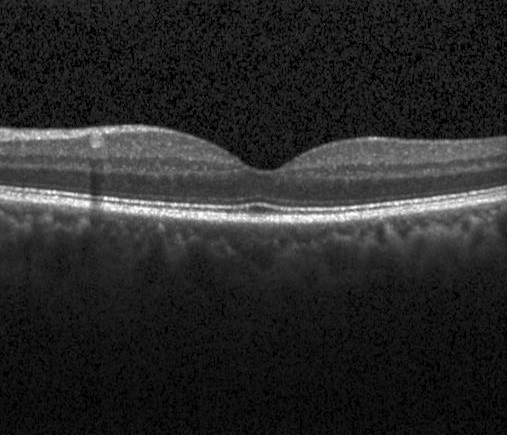
\includegraphics[width=0.5\linewidth]{figimages/Normal_eye.jpg}
\caption{OCT Scan of a Normal eye} 
\label{fig:OCT}
\end{figure}

\subsection{Time-domain Optical Coherence Tomography}
\vspace{1em}
In TD-OCT, the light beam gets divided into two parts: the sample beam and the reference beam. The retinal tissue gets struck by the sample beam and the light beam that is reflected after striking the tissue being imaged, is compared to the reference beam. The difference in time between the light beams and the intensity of the reflected light is used to visualize the retinal structure and its layers.

\subsection{Spectral-domain Optical Coherence Tomography}
\vspace{1em}
In SD-OCT, the light beams are split in a similar manner into the reference beam and sample beam. However, in SD-OCT, it is preferred to use a light source that can emit light with a broad range of spectrum. The sample beam is directed towards the retina tissue. The beam reflected after striking the tissue being visualized, is analysed using a spectrometer. The spectrometer measures the intensity and wavelength of the reflected light, and is used to visualize a 3-D image of the retinal structure and its layers. Out of the two measurement methods, the SD-OCT is found to be faster and better compared to conventional TD-OCT method. 

\section{Retinal Diseases}
There are many retinal diseases which can be detected using OCT scans. Some of the diseases are central serous retinopathy, macular hole, age-related macular degeneration (AMD), drusen, etc.\cite{OCTdiseases} The diseases which are being considered for classification in this research work are described in a detailed manner in the following sections:

\subsection{Age-related Macular Degeneration}
\vspace{1em}
AMD is an ocular condition which occurs at old age. AMD occurs at a much slower rate as compared to other retinal diseases. AMD has the following two types:
\begin{enumerate}
    \item \textbf{Dry AMD:} In dry AMD, the central region of retina, macula, gets thinner with age and slowly the person loses their central vision. This creates a blind spot at the centre of the eye.
    \item \textbf{Wet AMD:} In wet AMD, blood vessels grow abnormally under the retinal layer which causes fluids to leak, damaging the macula. Wet AMD is severe compared to dry AMD as it can cause complete loss of vison. Also, Wet AMD develops far more quickly than dry AMD.
\end{enumerate}

\begin{figure}[htb]
\centering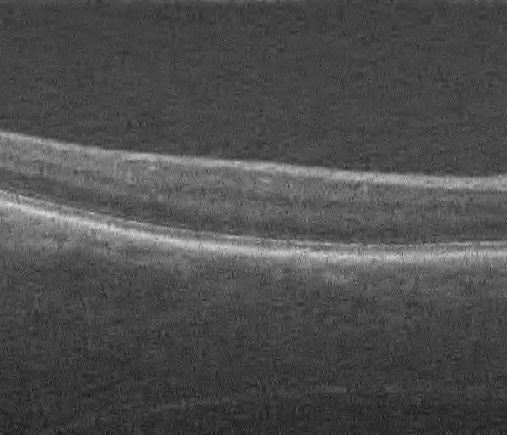
\includegraphics[width=0.5\linewidth]{figimages/AMD.jpg}
\caption{Age-related Macular Degeneration (AMD)} 
\label{fig:AMD}
\end{figure}

\subsection{Central Serous Retinopathy}
\vspace{1em}
CSR is the ocular disease in which fluids from choroid tissue layer leaks under the retina. It separates the retinal layer due to the cavity created, which causes blurry or unclear vision. CSR resolves usually in few months. Otherwise in some cases it may require medical attention.

\begin{figure}[htb]
\centering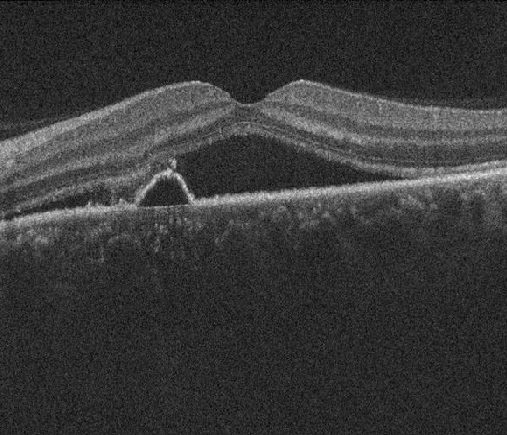
\includegraphics[width=0.5\linewidth]{figimages/CSR.jpg}
\caption{Central Serous Retinopathy (CSR)} 
\label{fig:CSR}
\end{figure}

\subsection{Macular Hole}
\vspace{1em}
When a tear is formed at macula due to being forced or stretched, the central vision of the eye blurs. This condition is called Macular Hole. Usually, macular hole is formed in the eyes with old age. The vitreous gel, which is the substance, which is filled between the lens and retina, wears off causing a macular hole to be generated.

\begin{figure}[htb]
\centering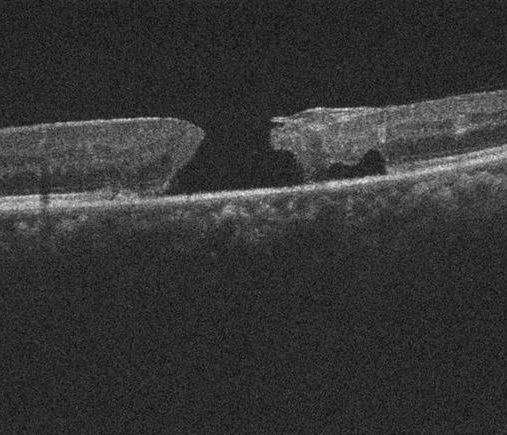
\includegraphics[width=0.5\linewidth]{figimages/MH.jpg}
\caption{Macular Hole} 
\label{fig:MH}
\end{figure}

\subsection{Drusen}
\vspace{1em}
Another ocular condition, Drusen is the deposition of yellow-coloured proteins and lipids or other waste materials under the retina. It may result in AMD, if left untreated. There are two types of Drusen:
\begin{enumerate}
    \item \textbf{Hard Drusen:} smaller particle deposits are termed as hard drusen. They do not in turn cause Age-related Macular Degeneration.
    \item \textbf{Soft Drusen:} large substances present in the eye are termed as soft drusen. They are related to Age-related Macular Degeneration.
\end{enumerate}
\begin{figure}[htb]
\centering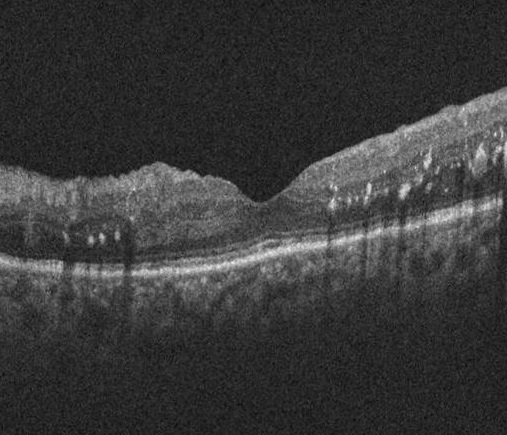
\includegraphics[width=0.5\linewidth]{figimages/Drusen.jpg}
\caption{Drusen} 
\label{fig:drusen}
\end{figure}

\section{Deep Learning}
Artificial Intelligence (AI) is the ability of computer systems or machine to mimic the human behaviour to identify or predict certain results including voice recognition, visual perception, prediction, etc. New advancements of modern age have found the use of AI at the centre of most of the industries. AI has various sub-domains including Natural Language Processing (NLP), Machine Learning, Robotics, etc.

\par
Machine learning is a sub-domain of AI which involves developing various algorithms which can predict certain outputs or classify inputs into different classes after training over given data. The main task of machine learning is to train the algorithms on data to learn and improve its performance. A typical machine learning task involves feature extraction from the given data, which is used in the algorithm as input to classify or predict the output. K-NN, Random Forest, Support Vector Machine (SVM) are few algorithms that have been used widely in Machine Learning.

\par
With new advancements, Deep Learning, which is a sub-field of machine learning has taken over and is being used for complex problems such as voice recognition, image classification, natural language processing etc. Deep Learning algorithms unlike machine learning, have complex multi-layered neural network structure which can automatically recognize patterns and features from the given raw data and provide a much higher accuracy as compared to the conventional methods. Deep learning algorithms may not require feature extraction step. The distinction between a machine learning and deep learning process is shown in Figure \ref{fig:machinedeeplearning}.

\begin{figure}[htb]
\centering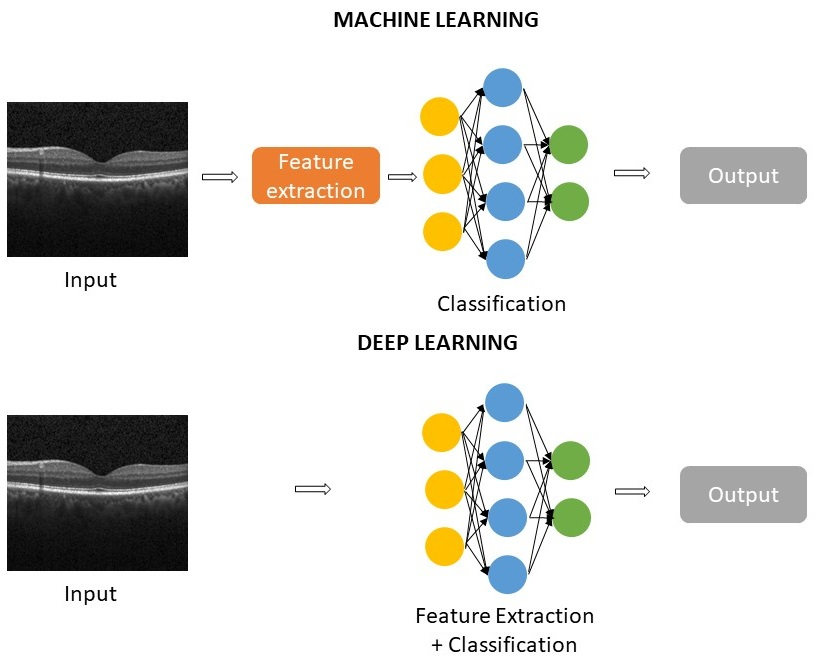
\includegraphics[width=0.85\linewidth]{figimages/Machine_Deep_Learning.jpg}
\caption{Comparison of Machine Learning and Deep Learning approaches} 
\label{fig:machinedeeplearning}
\end{figure}

\par
The use of Deep Learning for Artificial Intelligence problems has increased significantly in the past years with the rise in the access of more data and with increase of computational power. Graphical Processing Units (GPU) have been introduced, which is a type of processor which is used for complex calculations and parallel computations. The conventional machine learning training is carried out on CPU which is slower as compared to GPU computation speed.

\par
There are various types of deep learning network architectures which are designed to produce outputs specific to different set of problems. Two of the architectures which are important to this research work are described below:
\begin{enumerate}
    \item \textbf{Convolutional Neural Networks:} The CNN is a neural network architecture which is based on supervised learning, used mainly for classification tasks. A typical CNN consists of various layers including convolutional layers which are designed to extract image characteristics by sliding a kernel over image and create a different representation at each level, followed by other layers like pooling layers, batch normalization layers, and fully connected layers. The main advantage of using CNN over conventional machine learning method for classification is that CNN can learn the features and predict the class using raw image, whereas machine learning requires feature extraction before training to get better results.
    \item \textbf{Autoencoders:} Autoencoders \cite{Bank2020} are a specific type of neural network created to provide encoding and decoding of a given input to a desired form of output. Autoencoders are used for unsupervised learning problems including noise removal, reduce size to a smaller representation, automatic image colorization \cite{Singh2022}, etc. The Convolutional Autoencoders are a type of Autoencoders made using sequential convolutional layers for encoding and decoding of the input data. Zhang Y. \cite{Zhang} argued the use of Convolutional Autoencoders is best suited for images rather than linear autoencoders in their work. They compared the denoising and compression results of a convolutional and simple autoencoder in which the convolutional autoencoder outperformed the simple autoencoder. There are various use cases of Autoencoders out of which the Convolutional Autoencoders are mainly used for noise removal from images as shown in the research work by Yasenko \cite{DESSERT2020}. The Convolutional Autoencoders are trained with the actual image as the desired output and a slightly noisy image as the input. The autoencoder is trained with these input and output targets to provide a noise free output for a given image.
\end{enumerate}
\textbf{Hyperparameters:} Hyperparameters can be described as the changeable values in a deep learning training task which affects the algorithm and the results significantly. Hyperparameters are not learned by the algorithm but are provided or manually set by the user. It is necessary to choose the hyperparameter values carefully to obtain better result. Some of the hyperparameters are:
\begin{itemize}
    \item \textbf{Batch size:} Batch size is the number of training inputs which are fed in one iteration during training followed by weights updation. As the batch size increases, the convergence rate increases, however it requires a larger memory for computation. It is advised to start with a smaller batch size. \\
    With the decided batch size and size of input data, the total iterations per epoch is calculated.
    \begin{equation}
    \text{iterations} = \frac{\text{number of input data points}}{\text{batch size}}        
    \end{equation}
    \item \textbf{Epochs:} Epochs is each step of training, i.e., the number of times the training will loop over the data again and again to update the weights. In one epoch, the whole data is fed through the model and weights are updated, which is repeated in the next epoch. 
    
    \item \textbf{Loss Function:} It is a function which determines the overall loss a machine learning model makes during output prediction. It is calculated as the difference between the predicted and the true output. It is used to guide the optimizer algorithm to find the optimum value of weights which can achieve the minimum value of the loss function. The choice of loss function is specific to the given task. There are various loss functions including: \\
    Mean Square Error (MSE) Loss Function: MSE is generally used in regression tasks. It is the average squared difference between the predicted and the true output values.
    \begin{equation}
    MSE = \frac{1}{n}\sum_{i=1}^{n}(y_i - x_i )^2    
    \end{equation}
    where $y_i$ and $x_i$ are predicted and true output respectively. 

    Cross-entropy Loss Function: Similarly, the cross-entropy loss is used for classification tasks. It is the measure of difference between predicted probabilities and the true probabilities of the classes. It is calculated as
    \begin{equation}
        \text{Cross-entropy} = -\sum_{i=1}^nq_{i}\log(p_{i})
    \end{equation}
    where $q_i$ and $p_i$ are predicted and true probability respectively. 

    \item \textbf{Learning Rate:} It is the value which estimates the size of steps in which the weights are updated, or the step size with which the model converges. It is advised to begin with a small learning rate as a bigger value can cause the algorithm to overshoot and diverge from the minimum value. A smaller learning rate may increase the time of training but will reach an optimum value.
    
    \item \textbf{Optimizer:} Optimizer are the algorithm responsible for updating weights of a model during training step. The optimizer selected describes the way with which the weights will be updated to minimize the loss function. It works on the principle of back propagation. The simplest and most popular back propagation optimizer algorithm is Gradient Descent algorithm, also called as Stochastic Gradient Descent.

    \par
    Stochastic Gradient Descent (SGD): It modifies the model parameters according to the loss function gradient relative to the model parameters. It has a disadvantage, as it can get stuck in a local minimum and may fail to achieve the actual global minima.

    \par
    There are other optimizer algorithms available to overcome this and provide better results. Some of them are Adam optimizer, AdaGrad optimizer, RMSProp optimizer etc.
\end{itemize}

\section{The Process Flow of the Dissertation}
The following is the progression of this dissertation, through which the success of this work is achieved:

\begin{enumerate}
    \item \textbf{Chapter \ref{chapter:introduction} Introduction:} This is the introductory chapter of this dissertation. It explains the need of growing use of Artificial Intelligence in various sectors and its demand in medical sciences. It explains OCT, an optical scanning technique which is used for identification of various retinal diseases including Macular Hole, Age-related Macular Degeneration (AMD), Central Serous Retinopathy (CSR), and Drusen. It also sheds some light on the various AI methods involved in the research work like CNN, Autoencoders, and discuss various algorithms and hyperparameters and their importance that are involved in the training of these deep learning networks. 
    
    \item \textbf{Chapter \ref{chapter:literature} Literature Survey:} This chapter discusses various research and work that has been carried out in this field and which aligns with the research objectives. Additionally, it provides an insight on various methods that have been deployed or improved in this dissertation. The results of various methods have been obtained from this section to compare with the work in this dissertation.
    
    \item \textbf{Chapter \ref{chapter:proposedWork} Proposed Work:} This chapter discusses the methodology proposed in this research work. The research proposed utilizes a large collection of OCT images of each of these ocular conditions and develops a classifier to accurately classify the normal eye, and four other ocular diseases or conditions. The OCT images are processed and fed to a Convolutional Autoencoder network for noise removal. The denoised images are then enhanced or adjusted using Contrast Limited Adaptive Histogram Equalization (CLAHE).The enhanced images are normalized using the mean and standard deviation values. The image data is then trained on two different Convolution Neural Network (CNN) models. The first architecture is a simple CNN of five layers, and the other, a novel architecture, which utilizes bottleneck layer structures with convolutional layers. The purpose of this study is to enhance the existing detection method of diseases and provide a more efficient method for the ophthalmologists to utilize.
    
    \item \textbf{Chapter \ref{chapter:results} Experiments and Results:} In this chapter, the training and testing phase of the work is discussed. The training process is described along with the evaluation results obtained. Various evaluation parameters like Mean Square Error (MSE), Peak Signal-to-Noise Ratio (PSNR), Training and Validation Accuracy, Recall, Confusion matrix, F1 Score, etc. are used to evaluate the deep learning models’ performance. The training plots have also been visualized for the proposed methods.
    
    \item \textbf{Chapter \ref{chapter:conclusion} Discussion and Conclusion:} This chapter provides a comparison of the proposed method with the previous methods and its advantages over the previous approaches. It also concludes the research work. 
\end{enumerate}

% ------------------------ END -----------------------%
% ~
\vspace{8cm}
\begin{center}
$\qquad $ 
\end{center}
\vfill
~

 %chapter 2
\chapter{Literature Survey}
\label{chapter:literature} 
\noindent\rule{\linewidth}{2pt}

\section{Introduction}
Artificial Intelligence has been used in medical sciences for a long time and have advanced significantly. However, the introduction of AI in retinal diseases is quite recent. This chapter gives a summary of the recent works that have been carried out in this area. OCT is an interferometric scanning method which captures cross-sectional view of the biological tissues. It uses light’s coherent properties which have not been widely used previously in methods involving medical sciences.

\section{Study of Optical Coherence Tomography in Recent Publications}
Schmitt \cite{Schmitt} focused on the development of early OCT imaging methods and its introduction to the medical sciences. OCT provides a better structural and detailed view of the different sections of the eye as compared to confocal and bright field microscopes. The applications of OCT in ophthalmology have been recorded for the first time by Osiac et al. \cite{Osiac2011} and studied by Ţălu and Ţălu\cite{simonaDelia} in their research work. The authors focused specifically on AMD, providing a better insight into how OCT images are helpful for the identification of the diseases, the TD-OCT, and its progress to SD-OCT. Schmidt-Erfurth et al. \cite{Schmidt2017} explored and studied the use of OCT in monitoring and detection of AMD and early signs of AMD, Drusen and identify the progression of the diseases. The works of both the papers provided an analysis on why SD-OCT has been widely used for diagnosis, which provides a volumetric and cross-sectional view as compared to TD-OCT which gives only the cross-sectional view, i.e., a 2D perspective of the retina.

\section{Methodologies and Procedures Employed in Recent Publications}
A classification approach was published by Srinivasan et al. \cite{Srinivasan2014} based on Support Vector Machine \cite{708428} (SVM) which used multi-scale histograms as feature vectors to classify OCT images into AMD, DME and normal eyes. The work uses Block-matching and 3D Filtering \cite{6086619} (BM3D) for noise removal from SD-OCT images followed by resizing to a shape of 248 x 256. The retinal curvature of the image is flattened to approximate the curvature of all the images, as the curvature of each scan varies from patient to patient. The image is further cropped to 150 x 150 for feature extraction. The proposed method uses Support Vector Machine (SVM) for classification into multiple classes. It achieved high accuracy in detecting 100\% DME, 100\% AMD and 86.67\% of Normal eye images. Figure \ref{fig:Srinivasan2014} illustrates the process progression of the provided methodology.


\begin{figure}[htb]
\centering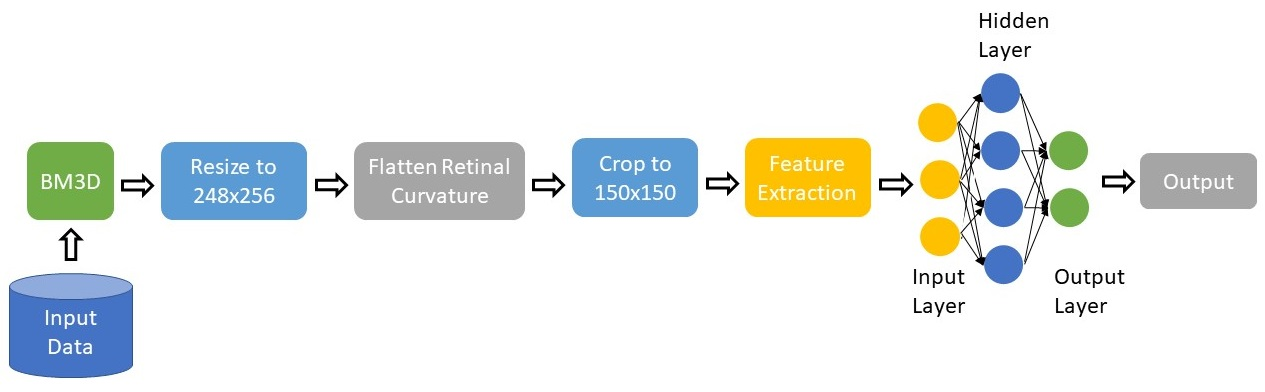
\includegraphics[width=\linewidth]{figimages/bm3dbased.jpg}
\caption{Process Flow of SVM based Classification Method proposed in \cite{Srinivasan2014}} 
\label{fig:Srinivasan2014}
\end{figure}

\par
Lemaître et al. \cite{Guillaume} focused on the classification of Diabetic Macular Edema (DME), amond the primary reasons of permanent vision loss in patients with diabetes. The OCT image data is de-noised using non-local means (NLM) filtering method, followed by flattening of the image curvature, like the flattening method used in the previous work. Further, the method uses feature extraction with five classical machine learning algorithms: k-NN, Logistic Regression, SVM, Random Forest, and Gradient Boosting for binary classification task. SERI dataset is used in the research work. For validation, specificity, sensitivity, confusion matrix, etc. parameters are visualized and assessed. Figure \ref{fig:Guillaume} visualizes all the steps of the given method.

\begin{figure}[htb]
\centering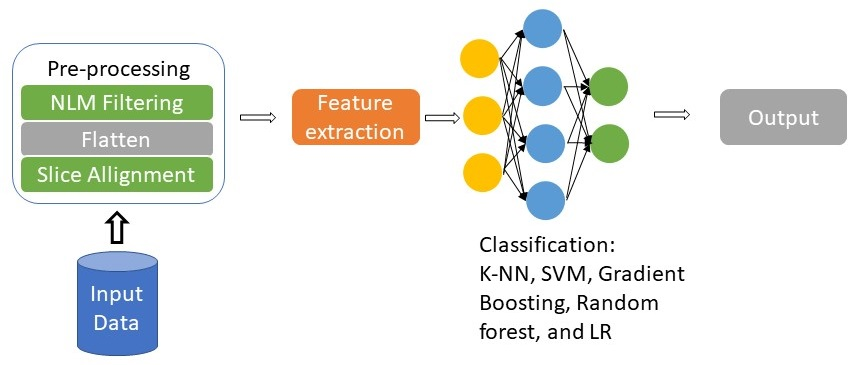
\includegraphics[width=\linewidth]{figimages/nlm6.jpg}
\caption{Classification Method proposed in \cite{Guillaume}} 
\label{fig:Guillaume}
\end{figure}

\par
Karri et al. \cite{Karri2017} introduced transfer learning approach for OCT-based classification of dieases in 3 classes, AMD, DME, and normal eye. The method uses pre-trained GoogleNet architecture for classification. The pre-processing phase consists of saturation removal, flattening followed by denoising. The pre-processed images are denoised using BM3D, followed by layer segmentation. The 3-channel input images fed to the GoogleNet are of dimensions 224x224. The Duke OCT dataset was used for training the said model and to evaluate the performance. The highest accuracy achieved was 96\%. This method proved that fine-tuned CNNs can be used to classify retinal pathologies effectively.

\begin{figure}[htb]
\centering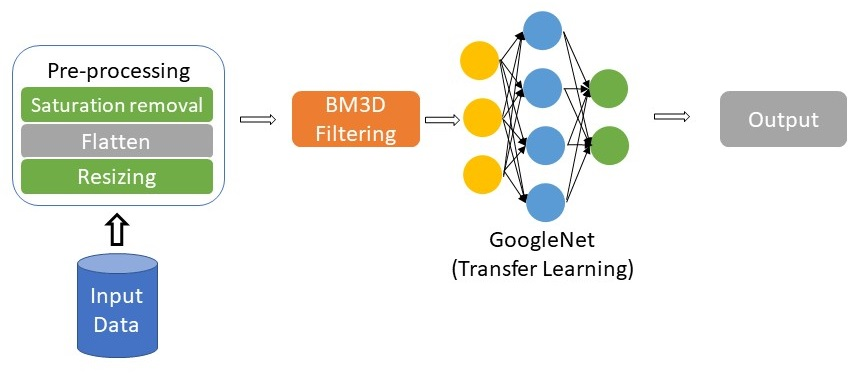
\includegraphics[width=\linewidth]{figimages/GoogleNet.jpg}
\caption{GoogleNet based method proposed in \cite{Karri2017}} 
\label{fig:Karri2017}
\end{figure}

\par
A binary classification method was given by Alsaih et al. \cite{Alsaih2017} for the detection of DME disease from SD-OCT images. The dataset was taken from SERI, Singapore consisting of 4,096 OCT images with normal and DME classes in ratio of 1:1. They diversified the data by selecting distinct lesions, i.e., abnormal tissue region in the Diabetic Macular Edema (DME) data sub-set. The proposed method used Principal Component Analysis \cite{WOLD198737} (PCA) in the classification pipeline with SVM resulting in a specificity of 87.5 and sensitivity of 87.5\%.

\par
Choi et al. \cite{Choi2017} used fundus photograph dataset of human eye from the publicly available dataset from Structured Analysis of the Retina (STARE) project for the CNN-based classification. MatConvNet \cite{VedaldiL14} architecture was used for the classification of retinal diseases. The dataset consisted of total of 10 classes including the normal human eye scans with each class containing around 1000 images each. The classification results were also obtained by using transfer learning method, specifically VGG19 architecture. Accuracy, RCI, and Kappa value were the parameters used for model evaluation. As the number of classes were increased to 10, the accuracy diminished to a low of 30.5\% on MatConvNet and a slightly better accuracy of 36.7\% on transfer learning method with VGG19 architecture. The process flow is described in Figure \ref{fig:Choi2017}.

\begin{figure}[htb]
\centering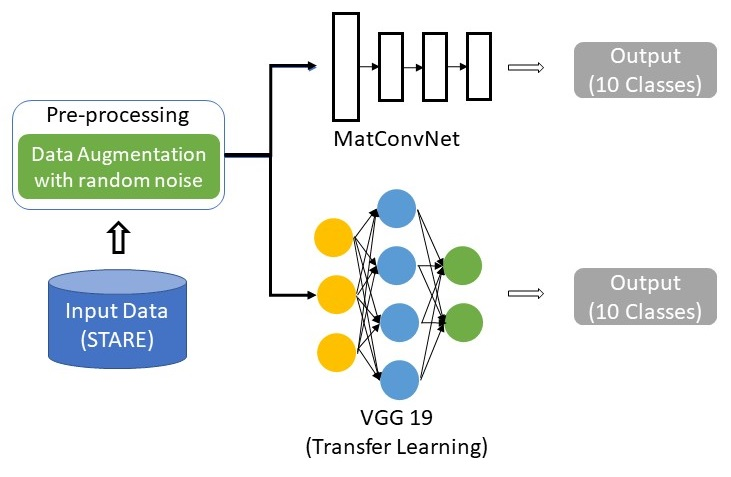
\includegraphics[width=\linewidth]{figimages/MatConvNet.jpg}
\caption{MatConvNet and VGG19 Classifier proposed in \cite{Choi2017}} 
\label{fig:Choi2017}
\end{figure}
\pagebreak
\par
In 2018, a novel method for classification of SD-OCT images of AMD, and DME was proposed by Hussain et al. \cite{Hussain2018}. The dataset consisted of 1,183 images of dimension 512x1024. The method involved segmentation of images for feature extraction and classification using various machine learning algorithms like SVM, Decision Tree, Random Forest out of which RF gave the best accuracy of 95\%. The proposed method can be visualized as below:

\begin{figure}[htb]
\centering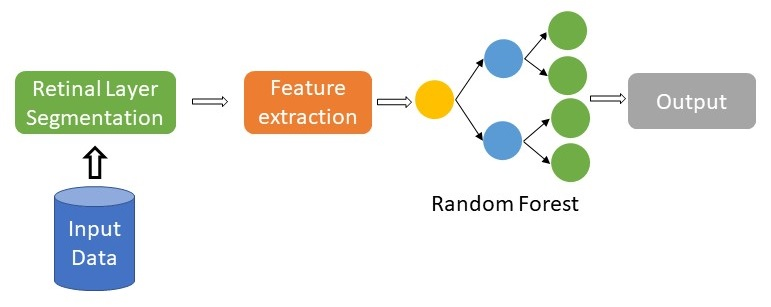
\includegraphics[width=\linewidth]{figimages/RandomForest.jpg}
\caption{Machine Learning based Classification of AMD and DME diseases} 
\label{fig:Hussain2018}
\end{figure}

\par
The research work proposed by Maetschke et al. \cite{Maetschke2019} involves a deep learning classification technique on unsegmented raw OCT scans, unlike its previous counterparts which used segmentation on OCT images before classification. The data includes scans from 624 patients having a total 1,110 images of healthy eye and 847 images of patients with Primary Open Angle Glaucoma (POAG). The images had a dimension of 200x1024. The evaluation metric used in this work was Area under the Receiver Operator Characteristic (AUC) curve. The proposed method classified a healthy eye with glaucomatous eyes using 3D CNN classifier with an accuracy of 94\%. This study proves that CNN can provide a good classification accuracy over raw unsegmented images in comparison to classical machine learning algorithms like k-NN, SVM, etc. The novel CNN architecture proposed in the above method consists of five 3D convolutional layers and a fully-connected layer. The architecture is described in the Figure \ref{fig:Maetschke2019}.

\begin{figure}[htb]
\centering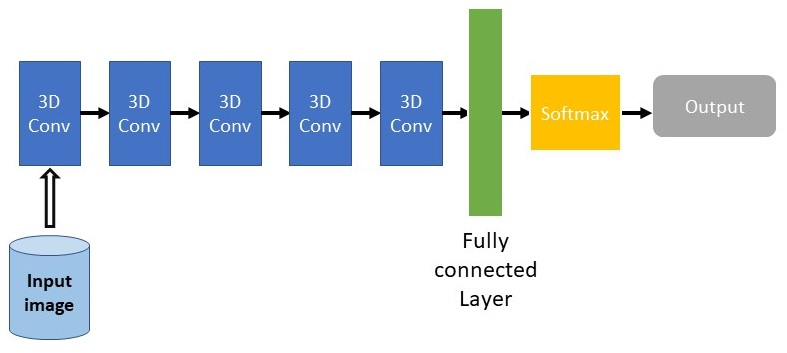
\includegraphics[width=\linewidth]{figimages/3DCNN.jpg}
\caption{3D CNN Architecture proposed in \cite{Maetschke2019}} 
\label{fig:Maetschke2019}
\end{figure}

\par
It is hard to automate the stacking of OCT images with a blurred layered structure and poor contrast.. Xiaoming et al. \cite{Xiaoming2019} resolved the issue by developing a novel OCT technique for detection that utilized complex Shearlet transforms. The evaluation data comprised of OCT images of Stargardt disease, dry AMD, and normal retinal macular region. The findings demonstrated that the complex Shearlet transform approach had been beneficial as it enabled the detection of more OCT image layers.

\par
Li et al. \cite{Li2019} devised and approach for classification of four ocular diseases including DME, CNV, Drusen and normal eye. The data was collected from Shanghai First People’s Hospital and Shanghai Zhongshan Hospital consisting of a total 15,573 OCT images, 3,786 in CNV, 3,238 in DME, 2,113 in Drusen, and 6,436 in normal eye. The evaluation parameters used in this method were accuracy, AUC curve, Kappa value, specificity, and sensitivity. The proposed method was based on transfer learning which employed a combination of 4 classification models which were formed using ResNet50 architecture, as shown in Figure \ref{fig:Li2019}, achieved an accuracy of 97.3\%.
\begin{figure}[htb]
\centering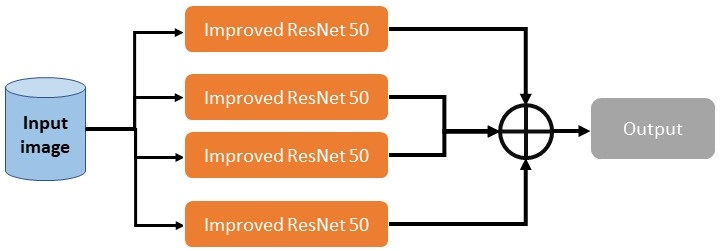
\includegraphics[width=\linewidth]{figimages/ResNet50.jpg}
\caption{ResNet50 Ensemble Classification Method \cite{Li2019}} 
\label{fig:Li2019}
\end{figure}

\par
One of the most recent and effective studies in the area of Retinal disease detection using SD-OCT images was carried out by Tayal et. al. \cite{Tayal2022}. The authors proposed three novel CNN architectures for the classification of DME, Drusen, CNV and normal eyes. The dataset used in this approach was taken from Mendeley Database having total 83,484 images. The images were then resized to 150x150 size and cropped to 128x128, where 128x128 being the input size for the CNN networks. The images were processed for noise removal using mean blur filter, contrast adjusted using Contrast Limited Adaptive Histogram Equalization (CLAHE) algorithm \cite{Sheet2022}, and edges were refined by drawing contours over them. The proposed method used 5-layered, 7-layered, and 9-layered convolutional neural networks which provided the highest accuracy of 96.5\%. This method's process flow is described in Figure \ref{fig:Tayal2022}.

\begin{figure}[htb]
\centering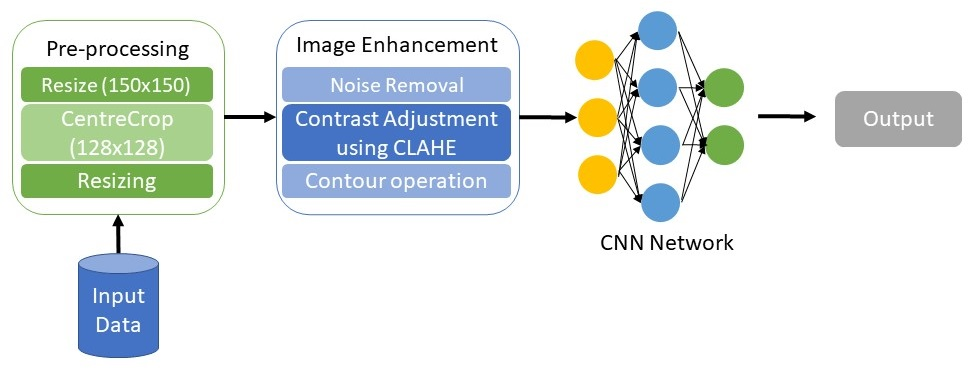
\includegraphics[width=\linewidth]{figimages/BasePaper.jpg}
\caption{Novel CNN architecture-based Classification method proposed in \cite{Tayal2022}} 
\label{fig:Tayal2022}
\end{figure}

\section{Problem Statement}
In accordance with World Health Organization (WHO) globally over 2.2 billion people have visual impairment out of which 1 billion cases could have been prevented if diagnosed early. In the modern world, it is essential to address this problem by devise ways for easy and error free detection of retinal or ocular diseases for diagnosis and treatment. 

\par
The increasing availability of medical data, combined with advancements in artificial intelligence (AI) technology, has led to the exploration of AI-based disease classification in medical sciences. In the present world, the use of advancing technology and application of Computer Science and Artificial Intelligence is growing drastically, especially in the biomedical sector for various purposes such as medical treatment, disease detection and diagnosis, etc. Artificial Intelligence has helped in reducing time consumed in diagnosis along with minimizing the scope of human errors. A sub-section of all the applications of Artificial Intelligence in Biomedical science is in Medical Image processing and disease diagnosis, i.e., the classification of diseases with minimal error, utilizing various image processing techniques and classification techniques. The scope of AI in ocular disease classification has increased significantly with advancements in eye-imaging techniques and artificial intelligence making it useful for ophthalmologists to devise a better way of determining the probability of a disease and to provide an immediate treatment. 

\section{Objectives}
To devise an improved approach for the classification of retinal diseases using OCT scans, we propose the following objectives which will be achieved in this dissertation work:
\begin{itemize}
    \item To identify and classify the OCT images into five categories including four retinal diseases- AMD, Drusen, Macular Hole, CSR, and normal human eye.
    \item Introduce a deep learning-based noise removal technique for denoising OCT images to remove speckle noise, which in turn will improve the model performance.
    \item Develop a novel deep learning architecture for the multi-classification problem.
    \item Measure the various evaluation parameters of the trained model like confusion matrix, accuracy, precision, recall, etc.
\end{itemize}
% ~
\vspace{8cm}
\begin{center}
$\qquad $ 
\end{center}
\vfill
~

% chapter 3
\chapter{Design, Setup and Methodology}
\label{chapter:methodology}
\noindent\rule{\linewidth}{2pt}

\section{Overview of the Experimental Pipeline}

The experimental pipeline of this dissertation can be partitioned into six stages, each with explicit input and output contracts, executed deterministically from a single random seed.

\begin{enumerate}[leftmargin=*]
\item \textbf{Data acquisition and SCP-based labelling.} Download PTB-XL via KaggleHub, parse \texttt{ptbxl\_database.csv}, derive binary MI versus NORM labels from the \texttt{scp\_codes} field and the \texttt{scp\_statements.csv} diagnostic-class mapping.
\item \textbf{Signal loading and per-record normalization.} Load each record's $(1000, 12)$ waveform from the \texttt{records100/} WFDB files at $100$\,Hz; apply per-record, per-lead $z$-score normalization.
\item \textbf{Patient-wise splitting.} Apply a deterministic two-stage \texttt{GroupShuffleSplit} over patient identifiers to obtain disjoint training (70\%), validation (15\%), and test (15\%) cohorts; assert disjointness at runtime.
\item \textbf{Base-model training.} Train three CNN base learners (\texttt{SimpleCNN}, \texttt{InceptionNet}, \texttt{ResNet1D}) independently from random initialization, with validation-AUC-based learning-rate scheduling and checkpoint selection.
\item \textbf{Embedding extraction and XGBoost training.} Extract penultimate-layer embeddings from the Inception anchor on the training, validation, and test cohorts; train an XGBoost classifier on the training embeddings with validation as the early-stopping monitor.
\item \textbf{Ensemble fusion, post-hoc tuning, and evaluation.} Combine the four predictors by validation-AUC-proportional weighting; optionally tune per-model thresholds and fit a logistic-regression meta-learner on out-of-fold validation predictions; evaluate on the held-out test cohort.
\end{enumerate}

The K-fold extension (\Cref{sec:kfold}) generalizes Steps 4 through 6 to a five-fold patient-wise resampling of the development cohort, producing fold-averaged predictions on the test cohort.

\section{The PTB-XL Dataset}

\subsection{Dataset Description}

The PTB-XL database~\cite{wagner2020ptbxl}, distributed via the PhysioNet repository~\cite{goldberger2000physiobank}, is the dataset used throughout this dissertation. Three properties make it suited to the present aim. First, it is large by ECG standards: \textbf{21{,}837} ten-second resting 12-lead recordings sourced from \textbf{18{,}885} distinct patients, collected in Germany between 1989 and 1996. Second, every record is shipped at two sampling rates, a 100\,Hz low-resolution version and a 500\,Hz high-resolution version, letting the experimentalist choose between fidelity and compute. The present work uses the 100\,Hz version exclusively. At this rate, the diagnostically relevant ST and T morphology is preserved (the Nyquist limit of $50$\,Hz is comfortably above the bandwidth in which ST changes manifest), the per-record tensor is just $(12, 1000)$, and a batch size of $64$ fits within the memory budget of a single Colab T4 instance. Third, each record carries clinical-grade annotations: two cardiologists independently assigned SCP-ECG diagnostic codes, and PTB-XL ships a curated mapping from those codes to the higher-level diagnostic classes (\texttt{NORM}, \texttt{MI}, \texttt{STTC}, \texttt{CD}, \texttt{HYP}) on which most binary and multi-label studies rely.

A record can carry multiple SCP codes simultaneously, which mirrors the multi-label nature of real clinical interpretation but, for a binary MI-vs-NORM study, requires the explicit selection rule described in the next subsection. The record-level metadata supplied alongside the waveform includes a patient identifier (the field on which patient-wise splitting depends), age, sex, recording site, recording date, and various technical fields (filter settings, electrode configuration, validating cardiologist's identifier). Of these, only the patient identifier is used downstream; the demographic fields are inspected for cohort-composition reporting but never fed into the model.

\subsection{Binary MI / NORM Label Construction}

Let $C(r)$ denote the set of SCP codes assigned to record $r$, and let $\mathcal{C}_{\mathrm{MI}}$ and $\mathcal{C}_{\mathrm{NORM}}$ denote, respectively, the sets of SCP codes whose diagnostic class is \texttt{MI} and \texttt{NORM} in \texttt{scp\_statements.csv}. The binary label $y(r)$ is defined as
\begin{equation}
y(r) = \begin{cases}
1 & \text{if } C(r) \cap \mathcal{C}_{\mathrm{MI}} \neq \emptyset \text{ and } C(r) \cap \mathcal{C}_{\mathrm{NORM}} = \emptyset, \\
0 & \text{if } C(r) \cap \mathcal{C}_{\mathrm{MI}} = \emptyset \text{ and } C(r) \cap \mathcal{C}_{\mathrm{NORM}} \neq \emptyset, \\
\bot & \text{otherwise (record is discarded)}.
\end{cases}
\end{equation}

The third (discard) branch excludes records with neither MI nor NORM codes (records dominated by ST/T changes, conduction disorders, or hypertrophy) and records that carry both MI and NORM codes simultaneously. The result is a clean binary problem in which the positive class is unambiguously infarction-positive and the negative class is unambiguously normal at the diagnostic level. The complete enumeration of MI codes used to populate $\mathcal{C}_{\mathrm{MI}}$ (14 codes covering anterior, anterolateral, anteroseptal, inferior, inferolateral, lateral, posterior, inferoposterior, inferoposterolateral, and subendocardial-injury patterns) and the single NORM code is given in \Cref{app:scp}.

\subsection{Demographic Composition of the Cohort}

\Cref{tab:demographics} reports the principal demographic characteristics of the working cohort and of each diagnostic class. The MI cohort is on average older than the NORM cohort by approximately a decade, with a mean age of $66.7$ years versus $53.4$ years, and is more heavily male ($63$\% versus $48$\% in NORM). Both patterns are consistent with the epidemiological literature on MI prevalence and reflect the biological reality that age and male sex are major modifiable and non-modifiable risk factors. These class-conditional demographic differences are partly informative for the classifier and partly a source of potential bias: a classifier that learns to predict MI from age alone, with no ECG signal, would already achieve substantial above-chance accuracy. The architecture choices in this dissertation reduce this risk by feeding only the ECG waveform to the network (no demographic inputs at the model boundary), but the underlying covariate structure of the cohort matters and is disclosed explicitly.

\begin{table}[h]
\centering
\caption{Demographic composition of the working cohort by diagnostic class. Ages are reported as mean $\pm$ standard deviation.}
\label{tab:demographics}
\begin{tabular}{lrrr}
\toprule
\textbf{Quantity}              & \textbf{MI cohort} & \textbf{NORM cohort} & \textbf{Overall} \\
\midrule
Records                        & 5{,}486            & 9{,}527              & 15{,}013         \\
Unique patients                & 4{,}932            & 8{,}521              & 13{,}453         \\
Records per patient (mean)     & 1.11               & 1.12                 & 1.12             \\
Age (years, mean $\pm$ SD)     & $66.7 \pm 11.8$    & $53.4 \pm 17.1$      & $58.3 \pm 16.6$  \\
Male fraction                  & 0.63               & 0.48                 & 0.53             \\
\bottomrule
\end{tabular}
\end{table}

\subsection{Cohort Statistics}

Applying the rule above to PTB-XL yields a working cohort of $15{,}013$ records from $13{,}453$ unique patients, with approximately $37$\% MI and $63$\% NORM at both record and patient level. \Cref{tab:cohort} summarizes the cohort.

\begin{table}[h]
\centering
\caption{Cohort statistics after SCP-based MI/NORM filtering of PTB-XL.}
\label{tab:cohort}
\begin{tabular}{lrr}
\toprule
\textbf{Quantity} & \textbf{Records} & \textbf{Unique patients} \\
\midrule
PTB-XL total                            & 21{,}837 & 18{,}885 \\
After MI / NORM filter (working cohort) & 15{,}013 & 13{,}453 \\
\quad of which MI (positive)            &  5{,}486 &  4{,}932 \\
\quad of which NORM (negative)          &  9{,}527 &  8{,}521 \\
\bottomrule
\end{tabular}
\end{table}

\section{Preprocessing Pipeline}

\subsection{Design Principles}

The preprocessing pipeline adopted in this dissertation is governed by three explicit design principles. \textit{Principle 1: minimize signal distortion.} Aggressive bandpass filtering, baseline-wander removal, and notch filtering can attenuate low-frequency ST-segment changes that are precisely the diagnostic information of interest. \textit{Principle 2: eliminate sources of leakage between training and evaluation data.} Per-record normalization is permitted because it is computed independently per sample; global normalization across the dataset is forbidden. Beat segmentation is forbidden because it creates highly correlated samples from the same patient. Synthetic oversampling is forbidden because it perturbs the empirical distribution. \textit{Principle 3: maintain reproducibility and protocol transparency.} Every preprocessing step is deterministic with fixed seeds; resulting train/validation/test indices are saved alongside checkpoints.

\subsection{Resampling, Standardization, and Channel Representation}

All experiments use the $100$\,Hz low-resolution version of PTB-XL. Each record is standardized to exactly 10 seconds ($1{,}000$ samples per lead); records longer than 10 seconds are truncated and shorter records zero-padded. No sliding-window segmentation, no fixed-stride cropping, and no time-domain augmentation are performed during preprocessing. Each 10-second record is treated as a single, atomic training instance. All twelve standard ECG leads (I, II, III, aVR, aVL, aVF, V1 through V6) are retained; signals are arranged in a channel-first tensor format $(12, 1000)$ at the dataset boundary.

\subsection{Per-Record \emph{z}-Score Normalization}

A single normalization is applied: per-record, per-lead $z$-score. For lead $\ell$ of record $r$ with samples $x_{r,\ell,t}$,
\begin{equation}
\hat{x}_{r,\ell,t} = \frac{x_{r,\ell,t} - \mu_{r,\ell}}{\sigma_{r,\ell} + \epsilon},
\qquad \epsilon = 10^{-8}.
\end{equation}
This normalization removes per-electrode amplitude scaling while preserving the relative morphology that carries the diagnostic information. Both $\mu$ and $\sigma$ are computed strictly within the record, so no information leaks across records.

\subsection{Filtering and Noise Handling: A Deliberate Absence}

The pipeline performs no explicit bandpass filtering, no baseline-wander removal, no power-line notch filtering, and no wavelet denoising. This is motivated by three considerations: modern CNN architectures with batch normalization~\cite{ioffe2015batch} suppress baseline drift implicitly; aggressive filtering risks attenuating slow ST-segment changes; and omitting heavy preprocessing makes the pipeline more robust to heterogeneous acquisition hardware. Pilot experiments comparing the pipeline with and without a 0.5--45\,Hz Butterworth bandpass showed no measurable AUC benefit from filtering.

\subsection{Augmentation Strategy}

For the canonical production pipeline (which produces the headline numbers of this thesis), no augmentation is applied; class imbalance is instead handled via a positive-class weight in the BCE loss. For the exploratory comparative study (the \texttt{titan/}, \texttt{ensemble/}, and \texttt{sota/} approach folders that pre-date the canonical pipeline), two mild augmentations were used during training: additive Gaussian noise with $\sigma = 0.01$ on all leads, and MI-class time scaling with factors uniformly in $[0.95, 1.05]$. Augmentation, where used, was strictly post-split and training-only.

\section{Patient-Wise Splitting Protocol}

The single most important methodological decision in this dissertation is to split data at the \textit{patient} level rather than at the record or beat level. The splitting routine is a deterministic two-stage \texttt{GroupShuffleSplit} from scikit-learn~\cite{pedregosa2011scikit}, parameterized by the patient-identifier array.

\Cref{lst:split} gives the pseudocode. The first stage holds out $15$\% of patients as the test cohort. The second stage further splits the remaining $85$\% into approximately $70$\% training and $15$\% validation. Disjointness of patient identifiers between all three splits is verified at runtime by set-theoretic assertions; the program aborts if any patient appears in more than one split. Random seeds are fixed at $42$ and $43$ for the two stages, so the partition is bit-reproducible across runs.

\begin{lstlisting}[caption={Patient-wise splitting routine (from \texttt{approaches/mi\_detection\_prod/data.py}).}, label={lst:split}]
def patient_wise_split(groups, test_frac, val_frac, seed):
    n = len(groups)
    all_idx = np.arange(n)

    gss1 = GroupShuffleSplit(n_splits=1, test_size=test_frac,
                              random_state=seed)
    trainval_idx, test_idx = next(gss1.split(all_idx, groups=groups))

    rel_val = val_frac / (1.0 - test_frac)
    gss2 = GroupShuffleSplit(n_splits=1, test_size=rel_val,
                              random_state=seed + 1)
    tr_rel, va_rel = next(
        gss2.split(trainval_idx, groups=groups[trainval_idx])
    )
    train_idx = trainval_idx[tr_rel]
    val_idx   = trainval_idx[va_rel]

    tr_p = set(groups[train_idx].tolist())
    va_p = set(groups[val_idx].tolist())
    te_p = set(groups[test_idx].tolist())
    assert tr_p.isdisjoint(va_p)
    assert tr_p.isdisjoint(te_p)
    assert va_p.isdisjoint(te_p)
    return train_idx, val_idx, test_idx
\end{lstlisting}

The resulting partition is summarized in \Cref{tab:split-stats}. The validation set is used exclusively for model selection, learning-rate scheduling, ensemble weight estimation, post-hoc threshold tuning, and meta-learner training. The test set is touched once at the end to compute the final reported metrics.

\begin{table}[h]
\centering
\caption{Patient-wise data partition used throughout this dissertation.}
\label{tab:split-stats}
\begin{tabular}{lrrr}
\toprule
\textbf{Split} & \textbf{Patients} & \textbf{Records} & \textbf{Approx.\ MI fraction} \\
\midrule
Training   & 9{,}417 & 10{,}511 & 0.37 \\
Validation & 2{,}018 &  2{,}233 & 0.38 \\
Test       & 2{,}018 &  2{,}269 & 0.37 \\
\midrule
Total      & 13{,}453 & 15{,}013 & 0.37 \\
\bottomrule
\end{tabular}
\end{table}

\section{Mathematical Foundations of the Models}
\label{sec:math-foundations}

This section formalizes the mathematical building blocks used by every model in this dissertation. The treatment is deliberately complete: subsequent architecture descriptions can then refer to these primitives by name without ambiguity.

\subsection{One-Dimensional Convolution}

A one-dimensional convolution layer with $K$ output channels, kernel size $k$, stride $s$, padding $p$, and dilation $d$ maps an input tensor $X \in \mathbb{R}^{C_{\mathrm{in}} \times T}$ to an output $Y \in \mathbb{R}^{K \times T'}$, where the temporal length is
\begin{equation}
T' = \left\lfloor \frac{T + 2p - d(k - 1) - 1}{s} \right\rfloor + 1.
\end{equation}
The output is computed channel-wise as
\begin{equation}
Y_{i,t} = b_i + \sum_{j=1}^{C_{\mathrm{in}}} \sum_{m=0}^{k-1} W_{i, j, m} \cdot X_{j,\, s\cdot t + d\cdot m - p},
\label{eq:conv1d}
\end{equation}
with learnable weight tensor $W \in \mathbb{R}^{K \times C_{\mathrm{in}} \times k}$ and bias $b \in \mathbb{R}^{K}$. The receptive field of a single convolution is $k$; stacked convolutions produce a receptive field that grows linearly with depth and exponentially with dilation.

For the TITAN base learners, all convolutions use stride 1 (with subsequent pooling for downsampling) except the ResNet1D stem, which uses stride 2, and the residual blocks at layers 2 through 4, which use stride 2 to halve the temporal dimension between layers.

\subsection{Batch Normalization}

Batch normalization~\cite{ioffe2015batch} normalizes activations using the batch-wise mean and variance, with two learnable parameters $\gamma$ and $\beta$ per channel:
\begin{equation}
\mathrm{BN}(x_{i}) = \gamma_i \cdot \frac{x_i - \mu_i^{(\mathcal{B})}}{\sqrt{\sigma_i^{2(\mathcal{B})} + \epsilon}} + \beta_i,
\end{equation}
where $\mu_i^{(\mathcal{B})}$ and $\sigma_i^{2(\mathcal{B})}$ are the per-channel mean and variance computed across the mini-batch $\mathcal{B}$, and $\epsilon = 10^{-5}$ is a numerical stabilizer. At inference time, running estimates of $\mu_i$ and $\sigma_i^2$ accumulated during training are used in place of batch statistics, so that single-record inference is deterministic.

\subsection{Rectified Linear Activation}

The ReLU non-linearity is
\begin{equation}
\mathrm{ReLU}(x) = \max(0, x).
\end{equation}
It is computationally cheap, does not saturate for positive inputs, and has well-understood gradient behaviour. All base learners use ReLU; alternatives such as GELU or SiLU were considered but did not improve validation AUC in pilot experiments.

\subsection{Residual Block}

A basic residual block~\cite{he2016deep} with input channels $C_{\mathrm{in}}$ and output channels $C_{\mathrm{out}}$ at stride $s$ computes
\begin{equation}
\mathcal{F}(X) = \mathrm{BN}\bigl(W_2 * \mathrm{ReLU}(\mathrm{BN}(W_1 * X))\bigr), \quad Y = \mathrm{ReLU}\bigl(\mathcal{F}(X) + \pi(X)\bigr),
\end{equation}
where $*$ denotes convolution, $W_1, W_2$ are kernel-3 convolutions (the first with stride $s$, the second with stride 1), and $\pi(\cdot)$ is the identity if $s=1$ and $C_{\mathrm{in}}=C_{\mathrm{out}}$, otherwise a $1\times 1$ projection convolution with stride $s$ followed by batch normalization. The residual connection enables training of deep networks by providing a direct gradient path from the loss to early layers.

\subsection{Inception Block}

The Inception block used in the TITAN \texttt{InceptionNet} has four parallel branches that operate on the same input and whose outputs are concatenated along the channel dimension:
\begin{align}
B_1 &= \mathrm{ReLU}(\mathrm{BN}(W_1 *_1 X)), \\
B_2 &= \mathrm{ReLU}(\mathrm{BN}(W_3 *_1 X)), \\
B_3 &= \mathrm{ReLU}(\mathrm{BN}(W_5 *_1 X)), \\
B_4 &= \mathrm{ReLU}(\mathrm{BN}(W_p *_1 \mathrm{MaxPool}_3(X))), \\
Y &= [B_1 ; B_2 ; B_3 ; B_4],
\end{align}
where $W_1, W_3, W_5$ denote kernel sizes 1, 3, and 5 respectively, $W_p$ is a $1\times 1$ projection after a $3\times 1$ stride-1 max-pool, and $[;]$ denotes channel-wise concatenation. Each branch produces $C_{\mathrm{out}}/4$ channels, giving a total of $C_{\mathrm{out}}$ output channels.

\subsection{Global Average Pooling}

For a tensor $Y \in \mathbb{R}^{C \times T'}$, global average pooling yields a vector $g \in \mathbb{R}^{C}$ with $g_c = \frac{1}{T'} \sum_{t=1}^{T'} Y_{c, t}$. GAP collapses the temporal dimension, providing translation invariance and reducing the parameter count of subsequent dense layers by a factor of $T'$ relative to a flatten-and-dense alternative.

\subsection{Self-Attention}

A scaled-dot-product attention~\cite{vaswani2017attention} layer with $h$ heads operates on an input sequence $X \in \mathbb{R}^{T \times D}$ by projecting it to queries $Q$, keys $K$, and values $V$ per head:
\begin{equation}
Q^{(\ell)} = X W^{(\ell)}_Q, \quad K^{(\ell)} = X W^{(\ell)}_K, \quad V^{(\ell)} = X W^{(\ell)}_V,
\end{equation}
and computing
\begin{equation}
\mathrm{Attn}^{(\ell)}(Q^{(\ell)}, K^{(\ell)}, V^{(\ell)}) = \mathrm{softmax}\!\left( \frac{Q^{(\ell)} {K^{(\ell)}}^\top}{\sqrt{d_k}} \right) V^{(\ell)}.
\end{equation}
The $h$ head outputs are concatenated and projected back to dimension $D$ by a learnable matrix $W_O$. Attention has complexity $\mathcal{O}(T^2 D)$, which for a 1000-sample ECG input is manageable but is the principal reason for the higher computational cost of attention-based and transformer-based variants explored in this work.

\subsection{Binary Cross-Entropy with Logits and Positive Weighting}

For binary classification with sigmoid output, the loss is
\begin{equation}
\mathcal{L}(\hat{y}, y) = -\bigl[\, w_{+} \cdot y \log\sigma(\hat y) + (1 - y) \log\bigl(1 - \sigma(\hat y)\bigr)\,\bigr],
\label{eq:bce-pos}
\end{equation}
where $\hat y$ is the network logit, $y \in \{0, 1\}$ the ground-truth label, $\sigma(\cdot)$ the logistic sigmoid, and $w_{+}$ a per-class weight. The numerically stable PyTorch implementation \texttt{BCEWithLogitsLoss(pos\_weight=$w_{+}$)} avoids explicit computation of the sigmoid.

\subsection{Adam Optimizer}

The Adam optimizer~\cite{kingma2015adam} maintains exponentially decaying running estimates of the first and second moments of per-parameter gradients,
\begin{equation}
m_t = \beta_1 m_{t-1} + (1-\beta_1) g_t, \qquad v_t = \beta_2 v_{t-1} + (1-\beta_2) g_t^2,
\end{equation}
and updates parameters as
\begin{equation}
\theta_{t+1} = \theta_t - \eta \cdot \frac{\hat m_t}{\sqrt{\hat v_t} + \epsilon},
\end{equation}
with bias-corrected estimates $\hat m_t = m_t / (1 - \beta_1^t)$ and $\hat v_t = v_t / (1 - \beta_2^t)$. The TITAN pipeline uses $\beta_1 = 0.9$, $\beta_2 = 0.999$, $\epsilon = 10^{-8}$, and $\eta_0 = 10^{-3}$, with $\eta$ subsequently controlled by the \texttt{ReduceLROnPlateau} scheduler.

\subsection{XGBoost Objective for Binary Classification}

The XGBoost classifier~\cite{chen2016xgboost} fits an additive ensemble of regression trees by minimizing
\begin{equation}
\mathcal{L}^{(t)} = \sum_{i=1}^{N} \ell\bigl(y_i, \hat y_i^{(t-1)} + f_t(\mathbf{z}_i)\bigr) + \Omega(f_t),
\end{equation}
where $\ell$ is the logistic loss for binary classification, $\hat y_i^{(t-1)}$ is the ensemble prediction up to round $t-1$, $f_t$ is the new tree added at round $t$, and $\Omega(f_t) = \gamma T + \frac{1}{2} \lambda \|w\|^2$ regularizes tree complexity ($T$ leaves, leaf weights $w$). A second-order Taylor expansion of the loss yields closed-form leaf weights and split scores, making each round computationally efficient. The TITAN pipeline trains XGBoost on the 128-dimensional Inception embeddings $\mathbf{z}$ with 600 trees, learning rate 0.05, and maximum depth 6.

\section{Model Architectures}
\label{sec:archs}

This section presents the architectures evaluated in this dissertation. All architectures receive the same input tensor of shape $(B, 12, 1000)$, where $B$ is the mini-batch size, and terminate in a single-logit head trained against binary cross-entropy with a positive-class weight. The three base learners of the TITAN ensemble (SimpleCNN, InceptionNet, ResNet1D) are described first; four additional architectures used in the comparative study are described thereafter.

\subsection{SimpleCNN: A Shallow Convolutional Baseline}
\label{sec:simplecnn}

\texttt{SimpleCNN} is a deliberately compact three-block convolutional network. Each block consists of a 1D convolution, batch normalization~\cite{ioffe2015batch}, a ReLU activation, and a max-pool layer of stride 2. Kernel sizes shrink from 7 (first block) to 5 to 3 (third block); filter counts grow $32 \to 64 \to 128$. After the third block, a global average pool collapses the temporal dimension to a 128-dimensional vector. A penultimate dense layer with ReLU activation maps this to a 128-dimensional embedding; a final linear layer projects to a single logit. Dropout $0.3$~\cite{srivastava2014dropout} precedes the head during training. The network has approximately 150\,k trainable parameters.

\subsection{InceptionNet: Multi-Scale Convolutions}
\label{sec:inception}

\texttt{InceptionNet} adapts the multi-branch convolution principle~\cite{szegedy2015going,ismail2020inception}. Each Inception block applies four parallel branches: a $1\times 1$ convolution, a $3\times 1$ convolution, a $5\times 1$ convolution, and a $3\times 1$ max-pool followed by a $1\times 1$ convolution. Each branch is followed by batch normalization and ReLU. Outputs are concatenated along channels. The full network is a $7\times 1$ stem (12 $\to$ 32 channels) followed by three Inception blocks with 32, 48, and 64 channels per branch respectively, max-pooled between blocks. A global average pool produces a 256-dimensional vector mapped to a 128-dimensional embedding by a penultimate dense layer. The network has approximately 0.5\,M parameters and serves as the \textbf{anchor} model of the TITAN ensemble: its penultimate embeddings are the input feature space for the XGBoost meta-classifier.

\subsection{ResNet1D: Deep Residual Network}
\label{sec:resnet1d}

\texttt{ResNet1D} is a one-dimensional adaptation of ResNet~\cite{he2016deep}. Each residual block contains two $3\times 1$ convolutions with batch normalization and ReLU, and a shortcut connection adding the block input to the second convolution's output. When channels or stride differ, a $1\times 1$ projection is used in the shortcut. The full network begins with a $7\times 1$ stem of stride 2 followed by a stride-2 $3\times 1$ max-pool. Four residual layers follow with channel counts $64 \to 128 \to 256 \to 512$ and stride 2 between layers; each layer contains two residual blocks. A global average pool produces a 512-dimensional vector mapped to a 128-dimensional embedding; dropout $0.3$ precedes the head. The network has approximately 4\,M parameters.

\subsection{Additional Architectures for the Comparative Study}

Three additional architectures are included in the comparative study reported in \Cref{chapter:results}.

\textit{ResNet1D with multi-head attention.} A self-attention module~\cite{vaswani2017attention} is inserted after the fourth residual layer and before the global average pool. The module treats each post-bottleneck temporal position as a token and applies a single multi-head self-attention layer with four heads. The attended sequence is added residually before pooling.

\textit{InceptionTime baseline at 250\,Hz.} A separate InceptionTime variant~\cite{ismail2020inception} uses bottleneck $1\times 1$ convolutions and kernel sizes $\{10, 20, 40\}$ at a sampling rate of $250$\,Hz, included for comparison with the $100$\,Hz InceptionNet.

\textit{Local/Global/Spectral Network (LGS-Net).} A dual-stream architecture combining a time-domain residual stream (with local-window attention) and a spectral stream operating on per-lead STFT magnitude spectrograms (with a 2D CNN), fused by concatenation before a dense head.

\textit{Compact Convolutional Transformer (CCT).} The convolutional-tokenizer plus Transformer-encoder design of Hassani et al.~\cite{hassani2021escaping}, adapted to 1D ECG with a two-block convolutional tokenizer (stride-2 $7\times 1$), a 4-block / 4-head / $D{=}128$ Transformer encoder, and a learnable class-pooling projection.

\Cref{tab:arch-summary} summarizes the architectures, their parameter counts, and their role in this study.

\begin{table}[h]
\centering
\caption{Summary of evaluated architectures.}
\label{tab:arch-summary}
\small
\begin{tabularx}{\textwidth}{l r l X}
\toprule
\textbf{Model} & \textbf{Params (M)} & \textbf{Family} & \textbf{Role in this study} \\
\midrule
SimpleCNN          & 0.15 & Pure CNN, shallow           & TITAN base learner; reference baseline \\
InceptionNet       & 0.5  & Multi-scale CNN             & TITAN \emph{anchor}; embeddings $\to$ XGB \\
ResNet1D           & 4.0  & Deep residual CNN           & TITAN base learner \\
ResNet+Attention   & 4.3  & Residual CNN + MHA          & Comparative study \\
InceptionTime      & 0.4  & Multi-scale CNN ($250$ Hz)  & Comparative study \\
LGS-Net            & 1.2  & Dual-stream time/spectral   & Comparative study \\
CCT                & 1.6  & Conv tokenizer + Transformer & Comparative study \\
\bottomrule
\end{tabularx}
\end{table}

\section{The TITAN Ensemble Framework}

\subsection{Motivation for Heterogeneous Ensembling}

Single-model ECG classifiers suffer from two recurrent failure modes that ensemble learning is well-suited to mitigate. First, individual deep networks are \textit{variance-dominated} in moderate-data regimes; averaging or stacking predictions from multiple base learners reduces this variance, in the spirit of bagging~\cite{breiman1996bagging}. Second, different architectures exhibit \textit{different inductive biases} and therefore make \textit{different kinds} of errors; combining them reduces the dependence on any single bias, in the spirit of stacked generalization~\cite{wolpert1992stacked}. The TITAN ensemble adds a third element: rather than fusing only the output probabilities of the base learners, it also fuses their \textit{latent representations}, by training an XGBoost~\cite{chen2016xgboost} classifier on the penultimate-layer embeddings of the Inception anchor. The intuition is that the pre-classifier embedding is a richer signal than the post-classifier scalar probability and that a gradient-boosted tree ensemble is well-suited to learn non-linear decision boundaries in that embedding space.

\subsection{TITAN Architecture and Data Flow}

TITAN (\textit{Three Independent Time-domain Architectures Network}) is structured around four predictors: an \textbf{anchor} (\texttt{InceptionNet}, producing both probability $p_{\mathrm{Inc}}$ and 128-dim embedding $\mathbf{z}_{\mathrm{Inc}}$); two \textbf{support} models (\texttt{SimpleCNN}, producing $p_{\mathrm{S}}$, and \texttt{ResNet1D}, producing $p_{\mathrm{R}}$); and an \textbf{embedding classifier} (\texttt{XGBoost} on $\mathbf{z}_{\mathrm{Inc}}$, producing $p_{\mathrm{X}}$). The three deep networks are trained independently on the same training cohort. After training, the Inception anchor is run in evaluation mode (\texttt{model.eval()}, dropout disabled, \texttt{torch.no\_grad()}) to extract embeddings for the training, validation, and test sets. The XGBoost model is then trained on the training embeddings, with validation embeddings as the early-stopping monitor and test embeddings withheld until final evaluation.

\subsection{Penultimate Embedding Extraction Discipline}

A subtle but important implementation detail is that the penultimate-layer embedding must be computed in a deterministic, dropout-free manner. Each architecture exposes a dedicated \texttt{.penultimate(x)} method that runs the trunk and the penultimate dense layer but not the final dropout or head. Combined with \texttt{model.eval()} (which switches batch normalization to inference mode) and \texttt{torch.no\_grad()} (which disables gradient bookkeeping), this guarantees bit-identical embeddings across multiple extractions of the same record. Earlier exploratory pipelines that did not follow this discipline produced different XGBoost training data on re-runs, a subtle source of non-determinism that was identified and removed in the canonical pipeline.

\subsection{Ensemble Fusion: Validation-AUC Weighted Averaging}

The four predictors are fused by a linear weighted average of their sigmoid probabilities. The weights are derived from validation-set AUC values $A_i$ of each predictor $i \in \{\mathrm{S}, \mathrm{Inc}, \mathrm{R}, \mathrm{X}\}$:
\begin{equation}
w_i = \frac{A_i}{\sum_{j} A_j}, \qquad
p_{\mathrm{TITAN}}(r) = \sum_i w_i\, p_i(r).
\end{equation}
This rule is intentionally simple. It avoids the overfitting risk of more elaborate learned-weight schemes and produces approximately uniform weights when all four predictors are similarly strong. The resulting weights are $(w_{\mathrm{S}}, w_{\mathrm{Inc}}, w_{\mathrm{R}}, w_{\mathrm{X}}) = (0.2503, 0.2505, 0.2488, 0.2504)$ for the canonical pipeline. A binary decision is obtained by thresholding $p_{\mathrm{TITAN}}$ at $0.5$ in the headline configuration; \Cref{chapter:results} also reports a post-hoc tuned-threshold result.

\subsection{Post-Hoc Logistic-Regression Meta-Learner}

A second, more expressive fusion is also implemented. A logistic-regression meta-learner takes the four base-model probabilities $(p_{\mathrm{S}}, p_{\mathrm{Inc}}, p_{\mathrm{R}}, p_{\mathrm{X}})$ as input and produces a scalar probability $p_{\mathrm{Meta}}$. The meta-learner is trained on the validation cohort, with five-fold patient-wise out-of-fold cross-validation used to derive a threshold that does not suffer from the in-sample optimism of training and tuning on the same fold. The fitted weights are
\[
p_{\mathrm{Meta}}(r) = \sigma\bigl(-4.4459 + 2.0494\, p_{\mathrm{S}} + 2.8445\, p_{\mathrm{Inc}} + 1.2088\, p_{\mathrm{R}} + 1.4699\, p_{\mathrm{X}}\bigr),
\]
where $\sigma(\cdot)$ is the logistic sigmoid. The Inception predictor receives the largest weight, consistent with its position as the embedding anchor.

\subsection{K-Fold Patient-Wise Ensemble Extension}
\label{sec:kfold}

For applications in which 1 to 2 additional percentage points of accuracy justify substantially increased training cost, a five-fold patient-wise extension is provided. The test set is held fixed (same patient-wise split as the canonical pipeline) and the combined training-plus-validation cohort is partitioned five ways using \texttt{GroupKFold} over patient identifiers. For each fold, three CNNs and one XGBoost classifier are trained on four folds and evaluated on the held-out fold, producing out-of-fold predictions on the development cohort and fold-averaged predictions on the test cohort. Both AUC-weighted averaging and logistic-regression meta-learning are then applied at the fold level. The K-fold ensemble produces 15 CNN checkpoints (3 architectures $\times$ 5 folds) and 5 XGBoost models in total; expected runtime is 60--90 minutes on a single T4 GPU.

\section{Training Algorithm in Detail}
\label{sec:training-algorithm}

The training procedure for each base learner is summarized as Algorithm-style pseudocode in \Cref{lst:train-loop}. The key design choices are: (i) the best checkpoint is selected by validation AUC at the end of each epoch, not by validation loss; (ii) learning-rate reduction and early stopping both monitor validation AUC, which keeps all model-selection signals on a patient-disjoint cohort; (iii) the loss-function positive weight $w_{+}$ is computed from the \textit{training} class distribution only, never from validation or test; and (iv) the validation AUC is recomputed on the full validation cohort after each epoch, so that early checkpoints are not biased by stochastic mini-batch statistics.

\begin{lstlisting}[caption={Training loop for a single base learner (paraphrased from \texttt{approaches/mi\_detection\_prod/train.py}).}, label={lst:train-loop}]
def train_one_model(model, train_loader, val_loader, n_pos, n_neg,
                    max_epochs=50, patience=8, lr=1e-3, wd=1e-4):
    pos_weight = torch.tensor([n_neg / max(n_pos, 1)])
    criterion = nn.BCEWithLogitsLoss(pos_weight=pos_weight.to(device))
    optimizer = optim.Adam(model.parameters(), lr=lr, weight_decay=wd)
    scheduler = optim.lr_scheduler.ReduceLROnPlateau(
        optimizer, mode='max', factor=0.5, patience=4, min_lr=1e-6)

    best_val_auc = -1.0
    best_state   = None
    epochs_since_improve = 0

    for epoch in range(max_epochs):
        # ----- train -----
        model.train()
        for x, y in train_loader:
            x, y = x.to(device), y.to(device)
            optimizer.zero_grad()
            logits = model(x)
            loss = criterion(logits, y)
            loss.backward()
            optimizer.step()

        # ----- validation AUC -----
        model.eval()
        val_logits, val_y = [], []
        with torch.no_grad():
            for x, y in val_loader:
                val_logits.append(model(x.to(device)).cpu())
                val_y.append(y)
        val_p = torch.sigmoid(torch.cat(val_logits)).numpy()
        val_y = torch.cat(val_y).numpy()
        val_auc = roc_auc_score(val_y, val_p)

        scheduler.step(val_auc)
        if val_auc > best_val_auc + 1e-6:
            best_val_auc = val_auc
            best_state = {k: v.detach().cpu().clone()
                          for k, v in model.state_dict().items()}
            epochs_since_improve = 0
        else:
            epochs_since_improve += 1
            if epochs_since_improve >= patience:
                break

    model.load_state_dict(best_state)
    return model, best_val_auc
\end{lstlisting}

The total training time for the three base learners on the canonical pipeline is approximately 12 to 18 minutes on a single Colab T4 GPU. Memory peak is approximately 4 to 6 GB. XGBoost training on the 128-dimensional Inception embeddings adds approximately 1 minute. Embedding extraction is approximately 30 seconds. Ensemble construction and reporting add a few seconds.

\section{Post-Hoc Threshold Tuning Algorithm}
\label{sec:threshold-tuning}

After training, the canonical pipeline runs a separate post-hoc tuning stage that does not modify any model weight. Two operations are performed.

\textit{Per-model threshold search.} For each of the four base predictors and for the AUC-weighted ensemble, the validation-set probabilities are sorted and a grid of candidate thresholds in $[0.01, 0.99]$ with step $0.005$ is evaluated. The threshold maximizing validation accuracy is selected and serialized. This threshold is then applied to the test-set probabilities of the corresponding predictor. The pseudocode is given in \Cref{lst:thr-tune}.

\begin{lstlisting}[caption={Accuracy-optimal threshold tuning on validation (\texttt{tune.py}).}, label={lst:thr-tune}]
def optimal_threshold(val_y, val_p, grid_lo=0.01, grid_hi=0.99, step=0.005):
    thresholds = np.arange(grid_lo, grid_hi + step, step)
    best_thr, best_acc = 0.5, -1.0
    for thr in thresholds:
        y_hat = (val_p >= thr).astype(int)
        acc = (y_hat == val_y).mean()
        if acc > best_acc:
            best_acc, best_thr = acc, float(thr)
    return best_thr, best_acc
\end{lstlisting}

\textit{Logistic-regression meta-learner.} A second-stage logistic regression is fit on the four-dimensional vector of base-model validation probabilities, $\mathbf{p}_{\mathrm{val}} = (p_{\mathrm{S}}, p_{\mathrm{Inc}}, p_{\mathrm{R}}, p_{\mathrm{X}})$. To avoid in-sample optimism from training and tuning on the same fold, the meta-learner threshold is chosen by five-fold patient-wise out-of-fold cross-validation on the validation cohort: for each fold, the meta-learner is fit on the other four folds and applied to the held-out fold, and the threshold is grid-searched on the resulting OOF predictions. The final meta-learner is then refit on the full validation cohort and applied, with the tuned threshold, to the test cohort.

The combined effect of these two operations is a modest but consistent accuracy improvement (approximately +0.6 percentage points on the TITAN ensemble; see \Cref{chapter:results}) at no additional training cost.

\section{Training and Optimization Protocol}

\subsection{Loss Function}

All deep networks are trained against binary cross-entropy on logits, with a positive-class weight to compensate for the residual class imbalance:
\begin{equation}
\mathcal{L} = -\frac{1}{N}\sum_{i=1}^{N} \bigl[ w_{+}\, y_i \log \sigma(\hat{y}_i) + (1 - y_i)\log(1 - \sigma(\hat{y}_i)) \bigr],
\end{equation}
where $\hat{y}_i$ is the network logit, $\sigma(\cdot)$ is the logistic sigmoid, and $w_{+}$ is the ratio of negative to positive training samples. This is the PyTorch \texttt{BCEWithLogitsLoss} with the \texttt{pos\_weight} parameter, which is numerically more stable than applying the sigmoid separately. XGBoost handles imbalance via the analogous \texttt{scale\_pos\_weight} parameter.

\subsection{Optimizer, Scheduling, and Stopping}

All deep networks are optimized using Adam~\cite{kingma2015adam} with $\eta = 10^{-3}$, $\beta_1 = 0.9$, $\beta_2 = 0.999$, weight decay $10^{-4}$. A \texttt{ReduceLROnPlateau} scheduler monitors the validation AUC and halves the learning rate when no improvement is observed for four consecutive epochs, with a floor of $10^{-6}$. Early stopping aborts training when no improvement in validation AUC has been observed for eight consecutive epochs. The maximum number of epochs is 50; in practice, all three base architectures converge in under 25 epochs. All training uses a batch size of 64.

\subsection{XGBoost Hyperparameters}

The XGBoost meta-classifier uses 600 trees, $\eta = 0.05$, maximum tree depth 6, row subsample 0.8, column subsample 0.8, the \texttt{hist} tree method on a single CPU thread (for determinism), AUC as the evaluation metric, and seed 42. Values were chosen to balance training time and predictive performance and to keep the XGBoost step deterministic.

\subsection{Reproducibility Harness}

A \texttt{set\_determinism(seed)} function is invoked at program start. It sets \newline \texttt{PYTHONHASHSEED} and \texttt{CUBLAS\_WORKSPACE\_CONFIG}, seeds the Python, NumPy, and PyTorch (CPU + CUDA) random number generators, forces cuDNN to deterministic mode, disables the cuDNN benchmark autotuner, and invokes \newline \texttt{torch.use\_deterministic\_algorithms(True)}. On a fixed CUDA toolkit and cuDNN version, the pipeline produces bit-identical outputs across multiple executions. The complete enumeration of seeds and other configuration constants is reproduced in \Cref{app:config}, and the inventory of released artefacts (checkpoints, embeddings, predictions, reports) is documented in \Cref{app:artefacts}.

\section{Evaluation Metrics and Protocol}

For each model, the following metrics are computed on the held-out test cohort: AUC; accuracy $(\mathrm{TP}+\mathrm{TN})/N$; sensitivity (recall) $\mathrm{TP}/(\mathrm{TP}+\mathrm{FN})$; specificity $\mathrm{TN}/(\mathrm{TN}+\mathrm{FP})$; precision $\mathrm{TP}/(\mathrm{TP}+\mathrm{FP})$; F1-score (harmonic mean of precision and recall); and the full $2\times 2$ confusion matrix. AUC is reported as the primary metric because it is threshold-independent. All other metrics are computed at the same fixed threshold ($0.5$ for the headline result; per-model accuracy-optimal thresholds for the tuned result, where the threshold is grid-searched on validation in $[0.01, 0.99]$ at step $0.005$).

No cross-validation is performed for the canonical pipeline; all metrics correspond to a single deterministic patient-wise split. The K-fold extension reports out-of-fold averages on the development cohort and fold-averaged predictions on the test cohort. The test set is touched once at the end of evaluation; no quantity computed on the test set is ever fed back into model selection, threshold setting, or ensemble weighting.

\section{Computational Environment}

The canonical pipeline was executed on a Google Colab T4 GPU instance with 16 GB GPU memory, with PTB-XL cached locally after an initial KaggleHub download (one-time cost approximately 1.7 GB). End-to-end runtime is approximately 15 to 25 minutes after dataset download. The K-fold pipeline requires approximately 60 to 90 minutes. Software stack: Python 3.10, PyTorch 2.x~\cite{paszke2019pytorch}, NumPy~\cite{pedregosa2011scikit}, scikit-learn~\cite{pedregosa2011scikit}, XGBoost 2.x~\cite{chen2016xgboost}, WFDB~\cite{xie2024wfdb}. All result artefacts (checkpoints, embeddings, predictions, configuration snapshots, JSON reports, Markdown tables, and confusion-matrix figures) are written to the \texttt{results/} directory and included in the released artefact bundle.

% ~
\vspace{8cm}
\begin{center}
$\qquad $ 
\end{center}
\vfill
~

% chapter 4
\chapter{Results and Discussion}
\label{chapter:results} 
\noindent\rule{\linewidth}{2pt}

\section{Introduction}
This chapter discusses the experimental setup used for training and evaluating the proposed architecture on OCT image data. The experimentation involves training the autoencoder and CNN classification networks to improve their performance and get desired results. Training refers to the process with which the machine learns parameters which are involved in the computation of results.

\section{Experimental Setup}
A local computer system is used for the training of neural network. The device has a RAM of 8 GB and an SSD Disk Space of 512 GB. The processor is Intel Core i5 10th generation with an NVIDIA GeForce GTX 1650 GPU. The GPU is used for parallel computation which helps in accelerating the training speed and time of complex models. The programming is done with Python 3.9 and PyTorch version 1.13.

\subsection{Training setup for Autoencoder}
\vspace{1em}
The Autoencoder has the hyperparameter initialization as shown in Table \ref{table: auto}, which has been chosen for optimal performance.

\subsection{Training setup for Five-layered CNN}
\vspace{1em}
The Five-layered CNN has the  hyperparameter initialization as shown in Table \ref{table: CNN},  which has been chosen for optimal performance.
\newpage

\begin{table}[ht]
\centering
\caption{Parameter initialization for Autoencoder}
\renewcommand{\arraystretch}{2} 
\begin{tabular}{|c|c|}
\hline
\textbf{Parameter} & \textbf{Value/type} \\  \hline
Weight initialization & Random \\ \hline
Input size & 256 x 256 \\ \hline
Loss criterion & MSE Loss \\ \hline
Optimizer & Adam Optimizer \\ \hline
Learning rate & 1 x $10^{-3}$ \\ \hline
Batch size & 16 \\ \hline
\end{tabular}
\label{table: auto}
\end{table}

\begin{table}[ht]
\centering
\caption{Parameter initialization for Five-layered CNN}
\renewcommand{\arraystretch}{2} 
\begin{tabular}{|c|c|}
\hline
\textbf{Parameter} & \textbf{Value/type} \\ \hline
Weight initialization & Random \\ \hline
Input size & 128 x 128 \\ \hline
Loss criterion & MSE Loss \\ \hline
Optimizer & Adam Optimizer \\ \hline
Learning rate & 5.5 x $10^{-5}$ \\ \hline
Batch size & 16 \\ \hline
\end{tabular}
\label{table: CNN}
\end{table}

\subsection{Training setup for Bottleneck CNN}
\vspace{1em}
The Bottleneck CNN has the following hyperparameter initialization as shown in Table \ref{table: bottleneck} which has been chosen for optimal performance.
\newpage
\begin{table}[ht]
\centering
\caption{Parameter initialization for Bottleneck CNN}
\renewcommand{\arraystretch}{2} 
\begin{tabular}{|c|c|}
\hline
\textbf{Parameter} & \textbf{Value/type} \\ \hline
Weight initialization & Random \\ \hline
Input size & 128 x 128 \\ \hline
Loss criterion & MSE Loss \\ \hline
Optimizer & Adam Optimizer \\ \hline
Learning rate & 1 x $10^{-5}$ \\ \hline
Batch size & 16 \\ \hline
\end{tabular}
\label{table: bottleneck}
\end{table}

\section{Results}
The summary of the three proposed models for noise removal and classification are shown as follows:
\newpage

\begin{figure}[H]
\centering
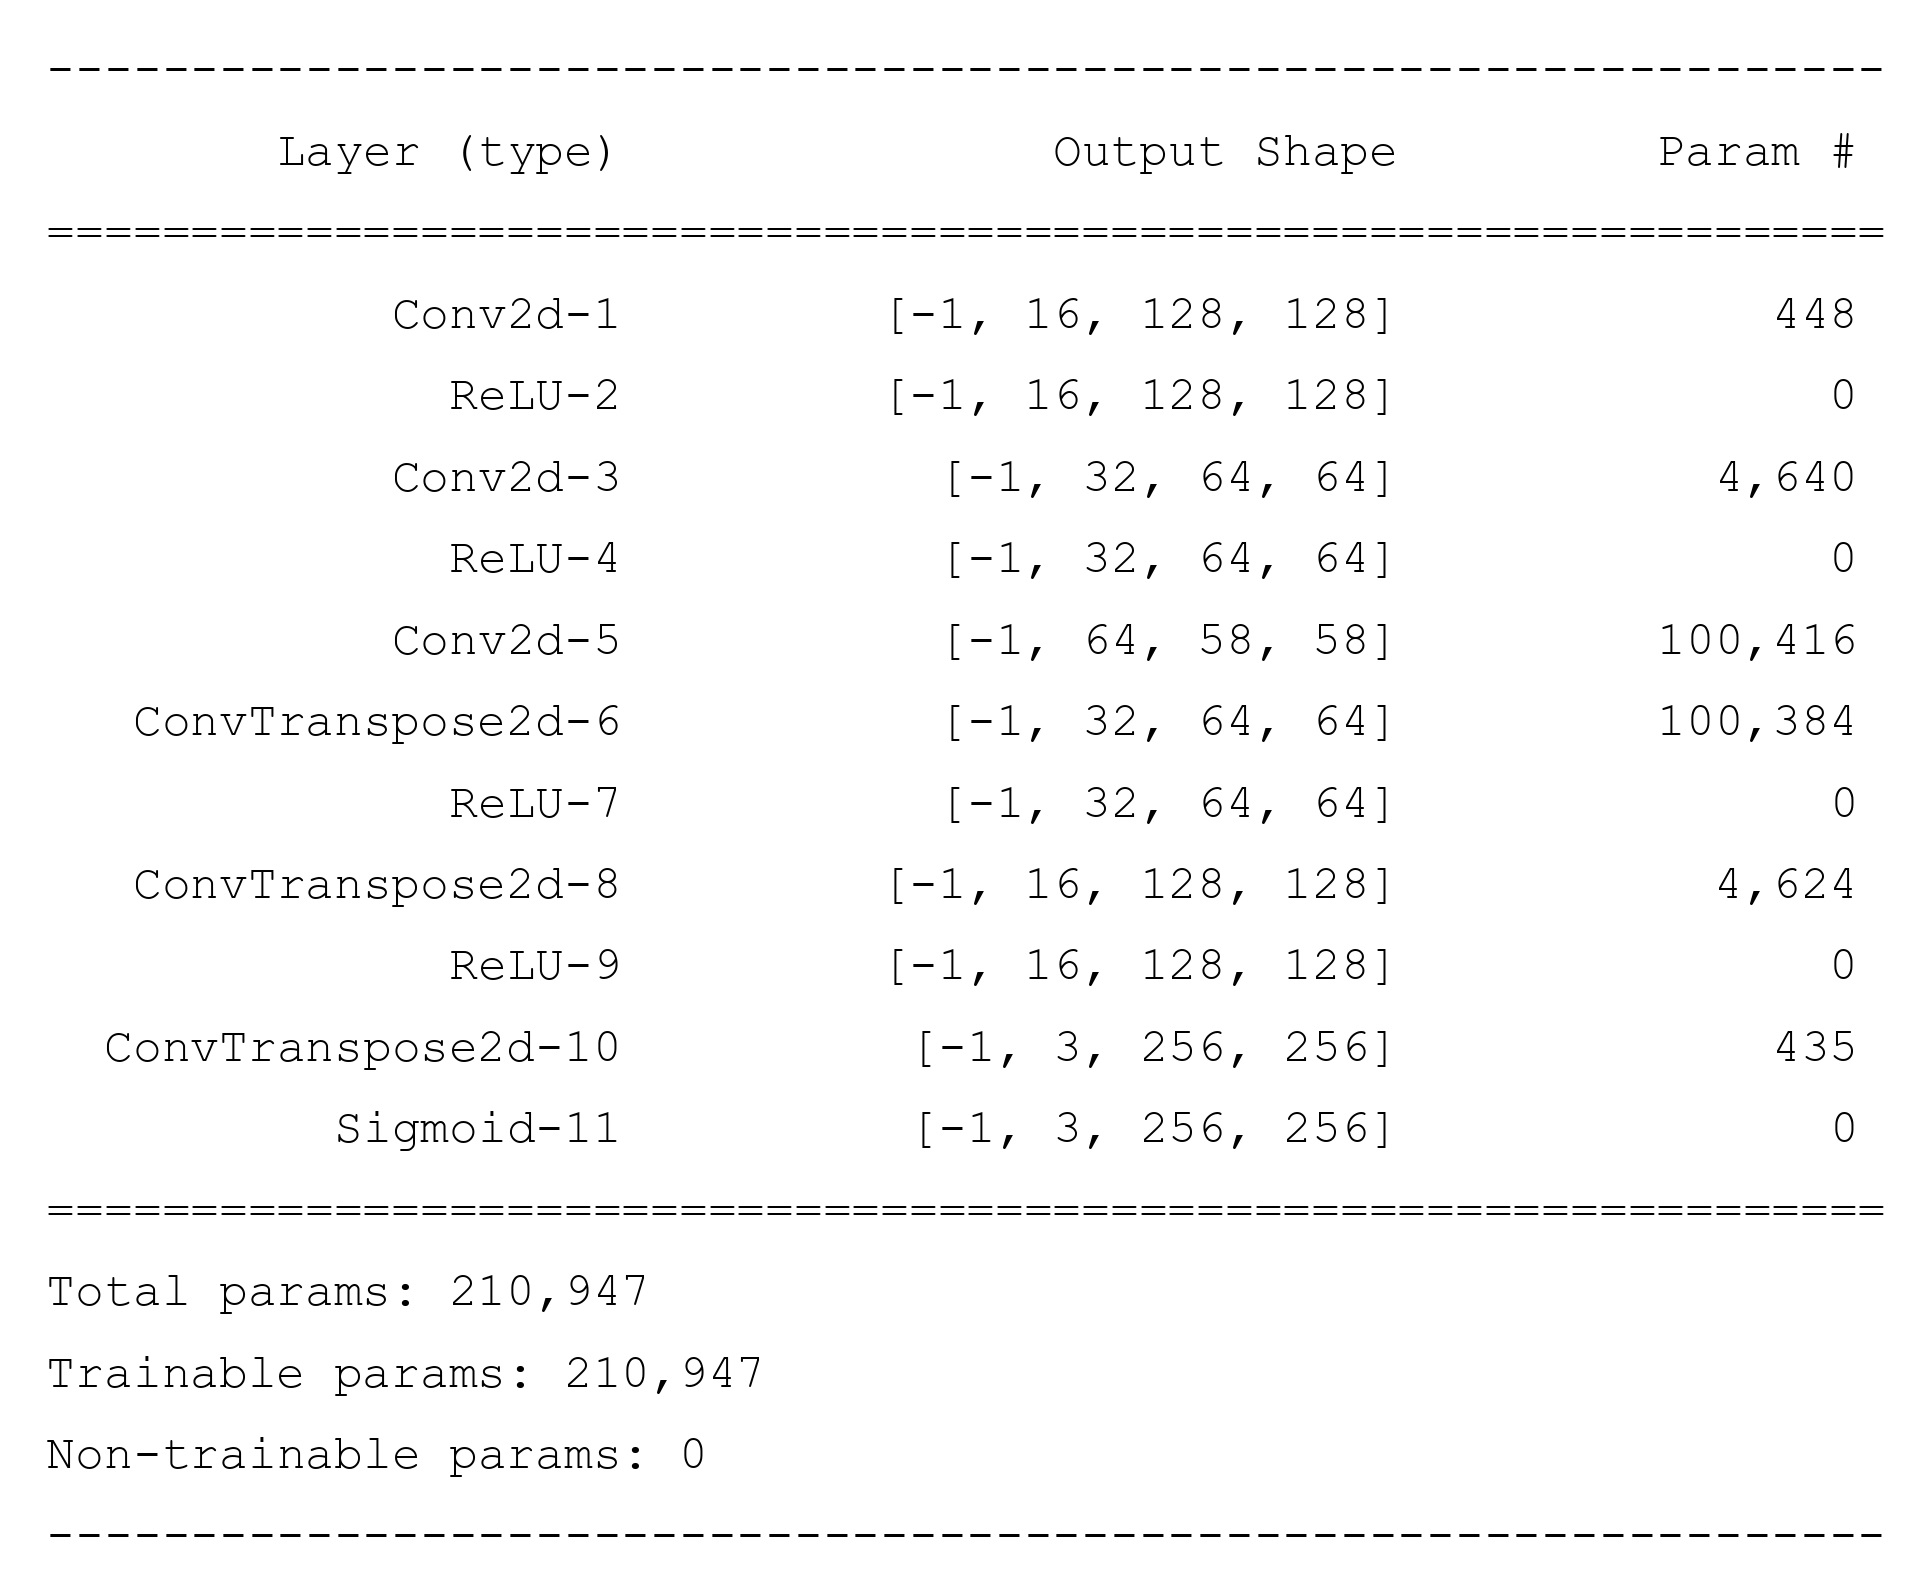
\includegraphics[width=\linewidth]{figimages/summaryAutoencoder.jpg}
\caption{Summary of Autoencoder model}
\label{fig: autoencoder summary}
\end{figure}


\begin{figure}[H]
\centering
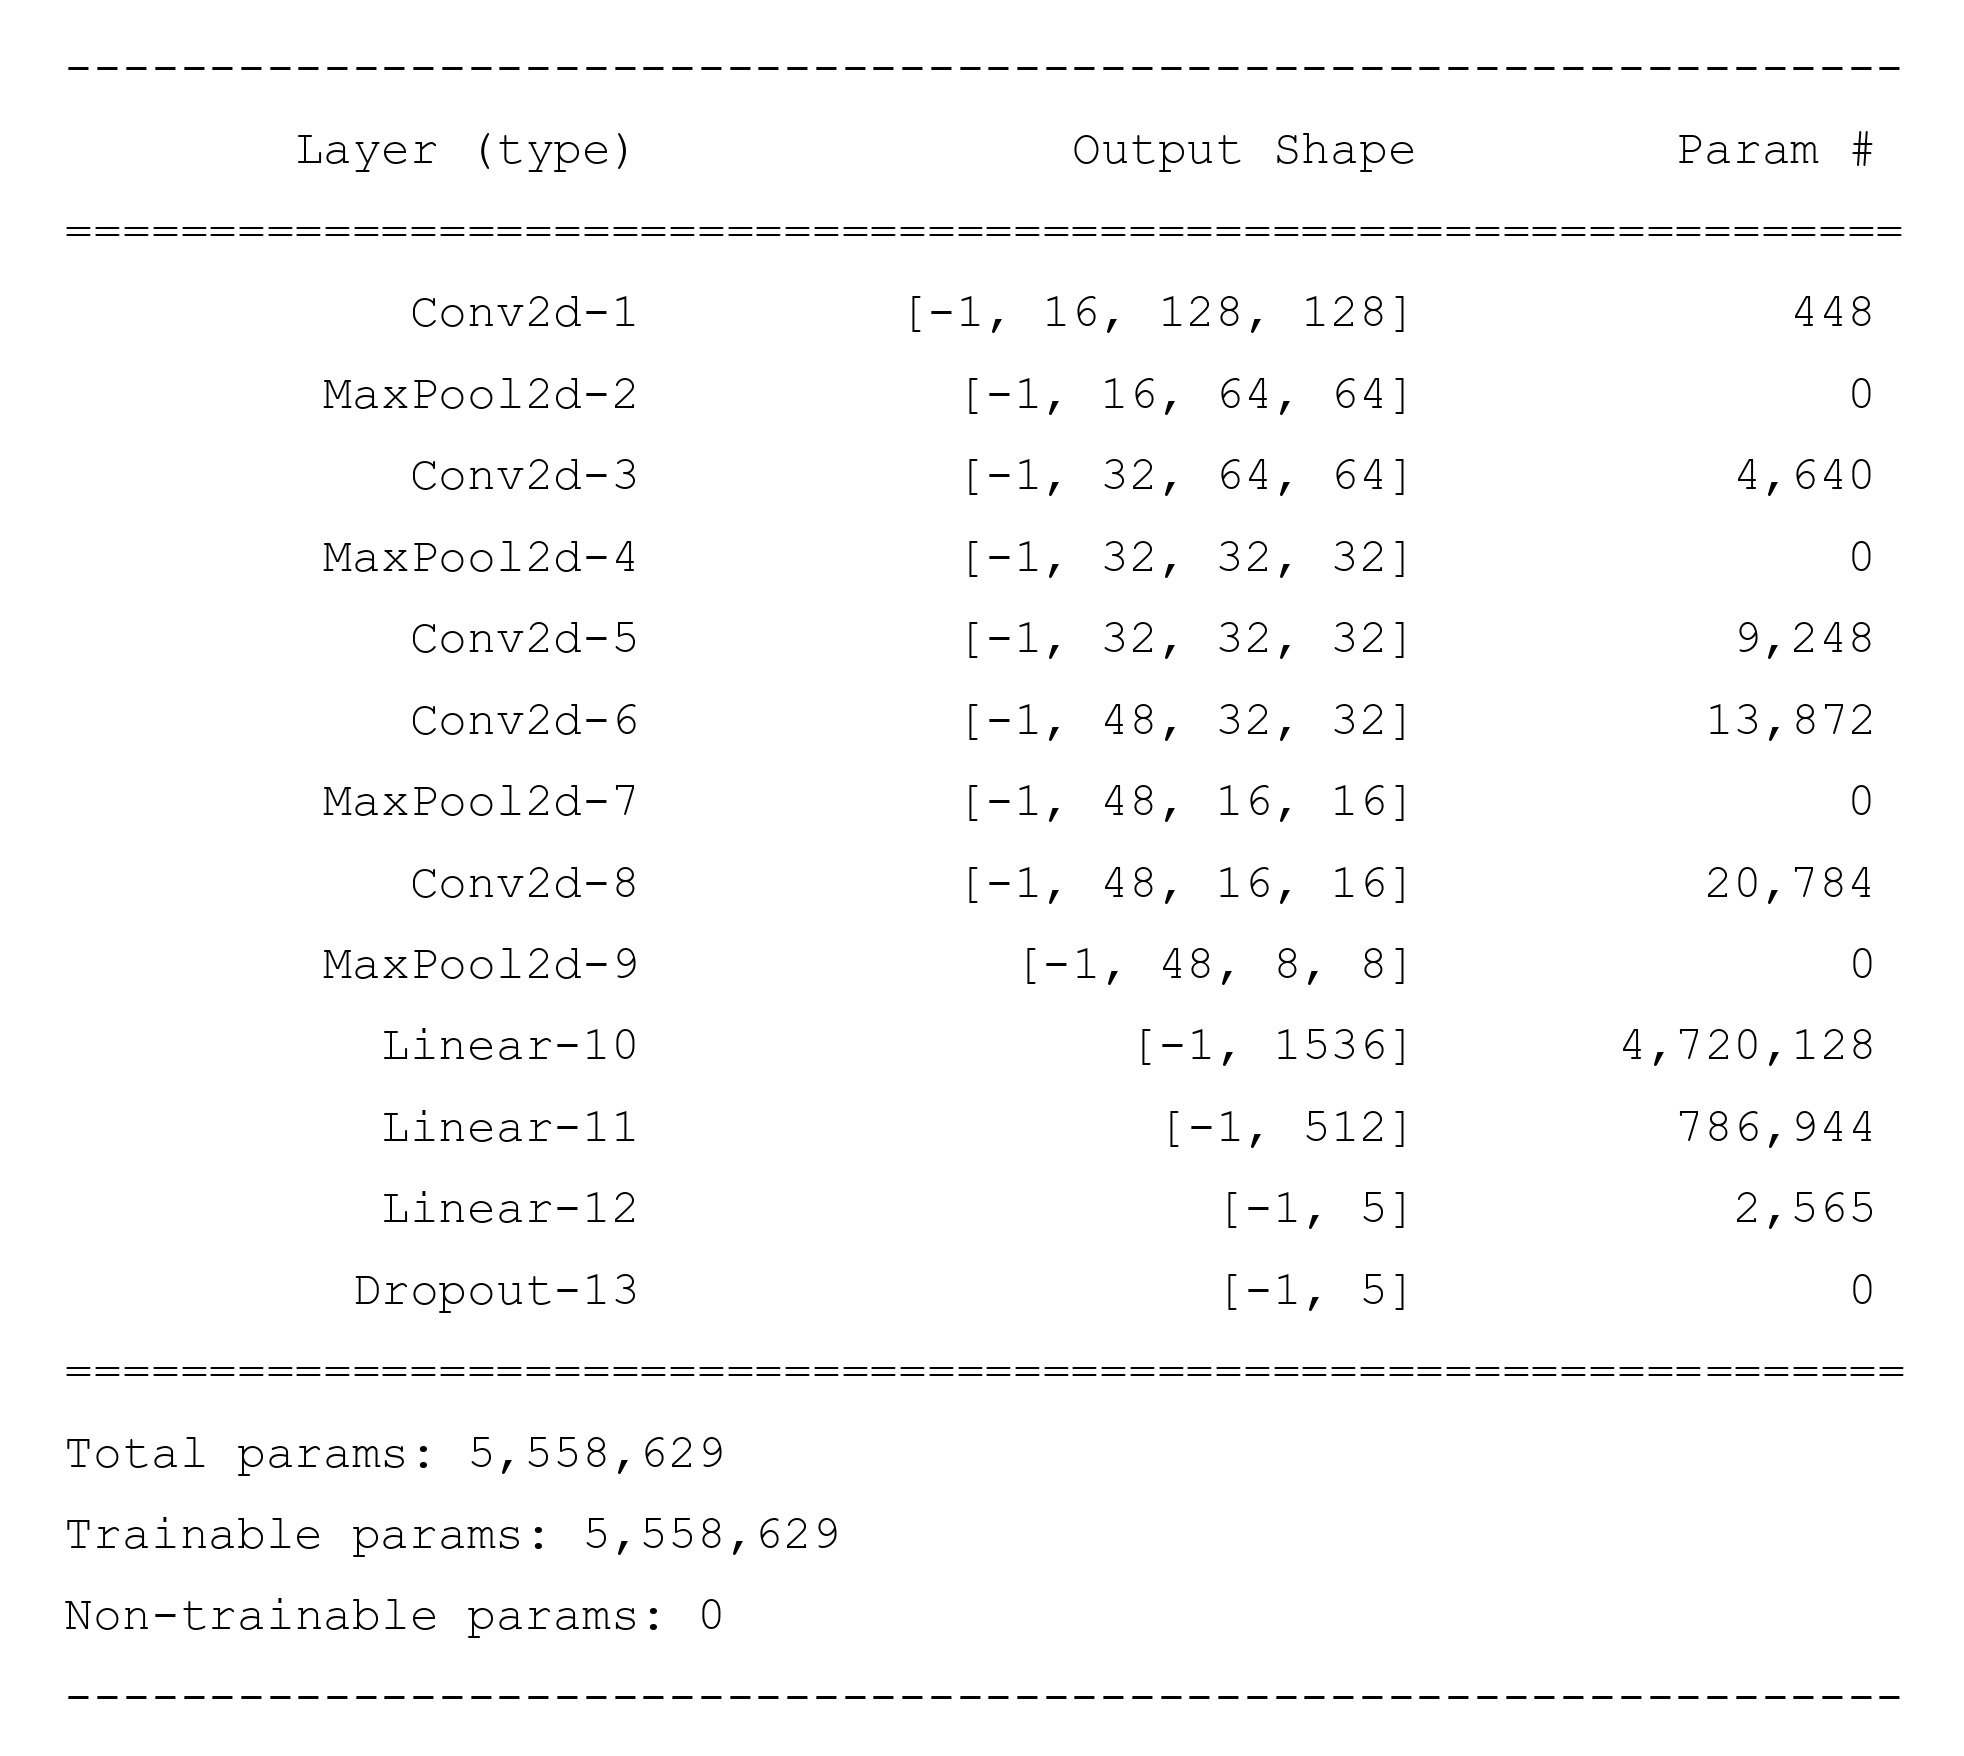
\includegraphics[width=\linewidth]{figimages/summary5Layered.jpg}
\caption{Summary of Five-layered CNN model}
\label{fig: 5CNN summary}
\end{figure}

\begin{figure}[H]
\centering
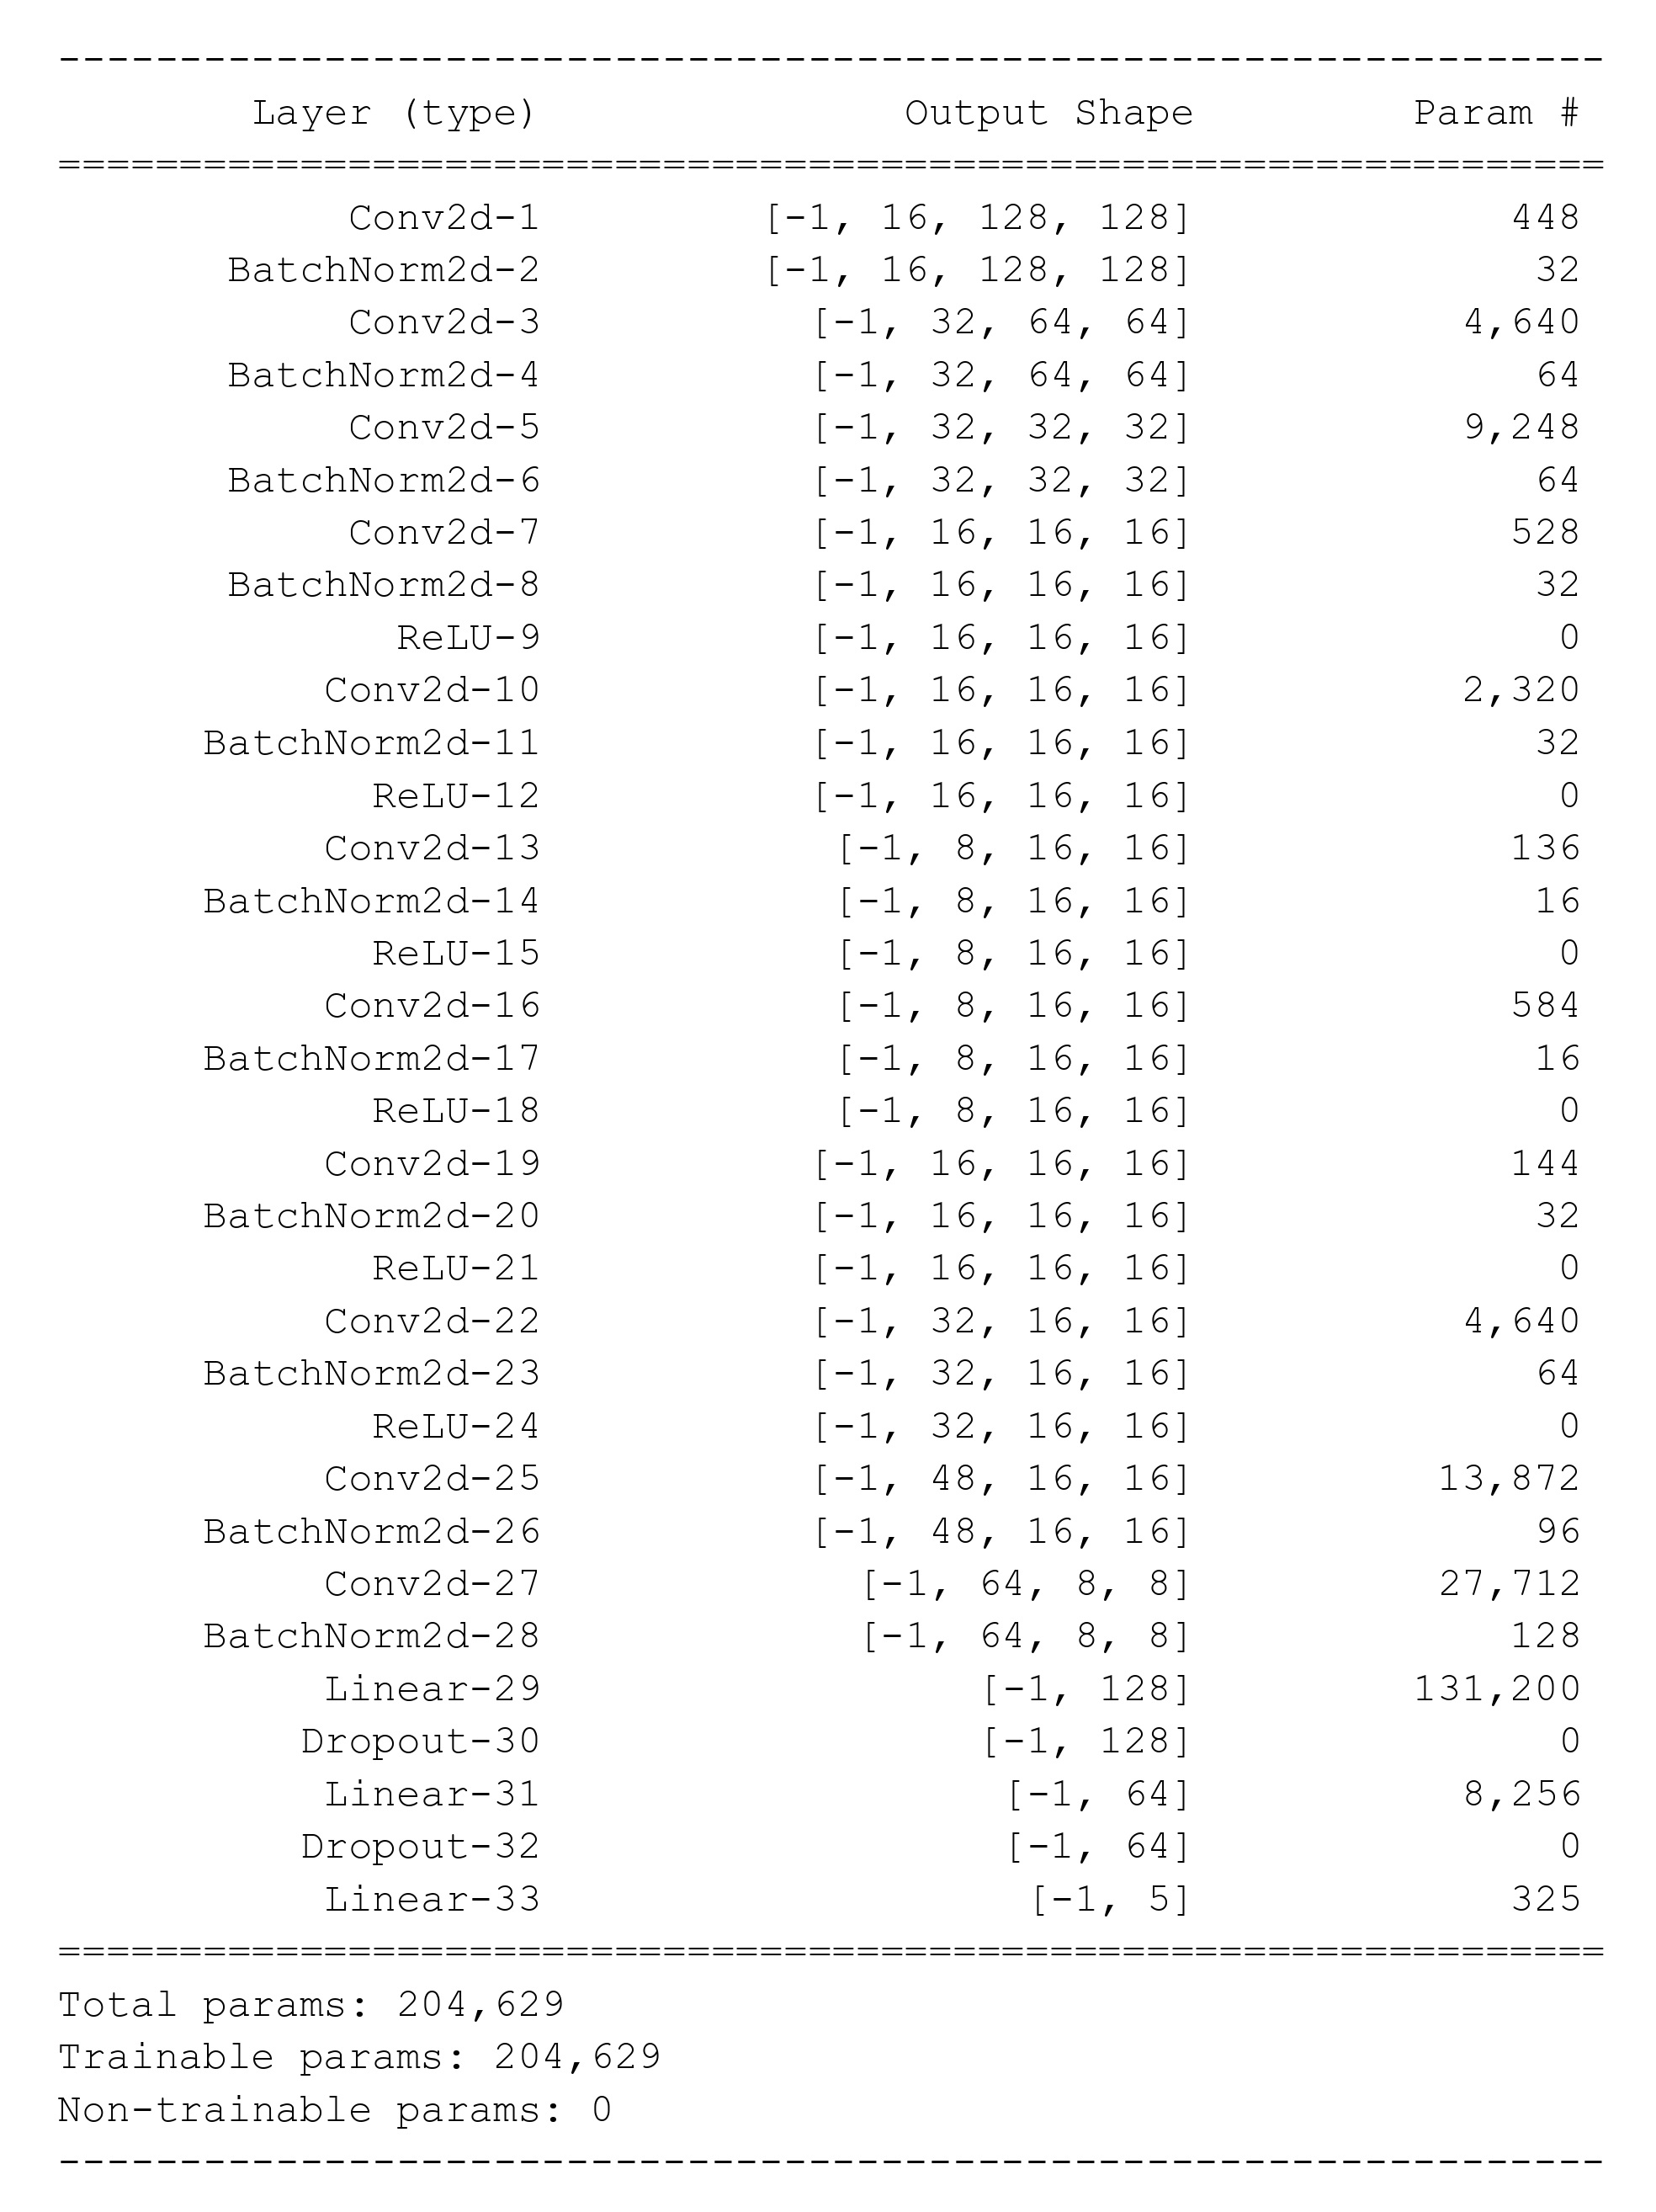
\includegraphics[width=\linewidth]{figimages/summaryBottleneck.jpg}
\caption{Summary of Bottleneck CNN model}
\label{fig: bottleneckSummary}
\end{figure}
\newpage

\subsection{Autoencoder}
\vspace{1em}
The PSNR and Mean Square Error plots during training of the Autoencoder have been shown in Figure \ref{fig: PSNR} and \ref{fig: MSE} respectively. The peak value of PSNR achieved is 27.324.

\begin{figure}[htb]
\centering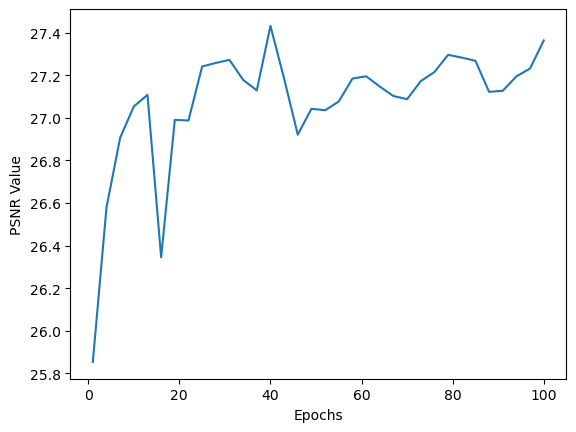
\includegraphics[width=0.7\linewidth]{figimages/PSNRplot.png}
\caption{PSNR Training Plot} 
\label{fig: PSNR}
\end{figure}

\begin{figure}[htb]
\centering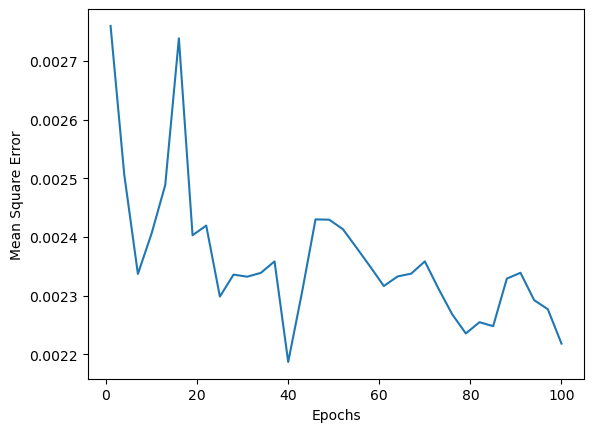
\includegraphics[width=0.7\linewidth]{figimages/MSEplot.png}
\caption{Mean Square Error plot during training} 
\label{fig: MSE}
\end{figure}

\par
The Figure \ref{fig: comparison} shows a comparison between the results obtained after noise removal and after applying the contrast adjustment using CLAHE on the denoised images.

\begin{figure}[htb]
\centering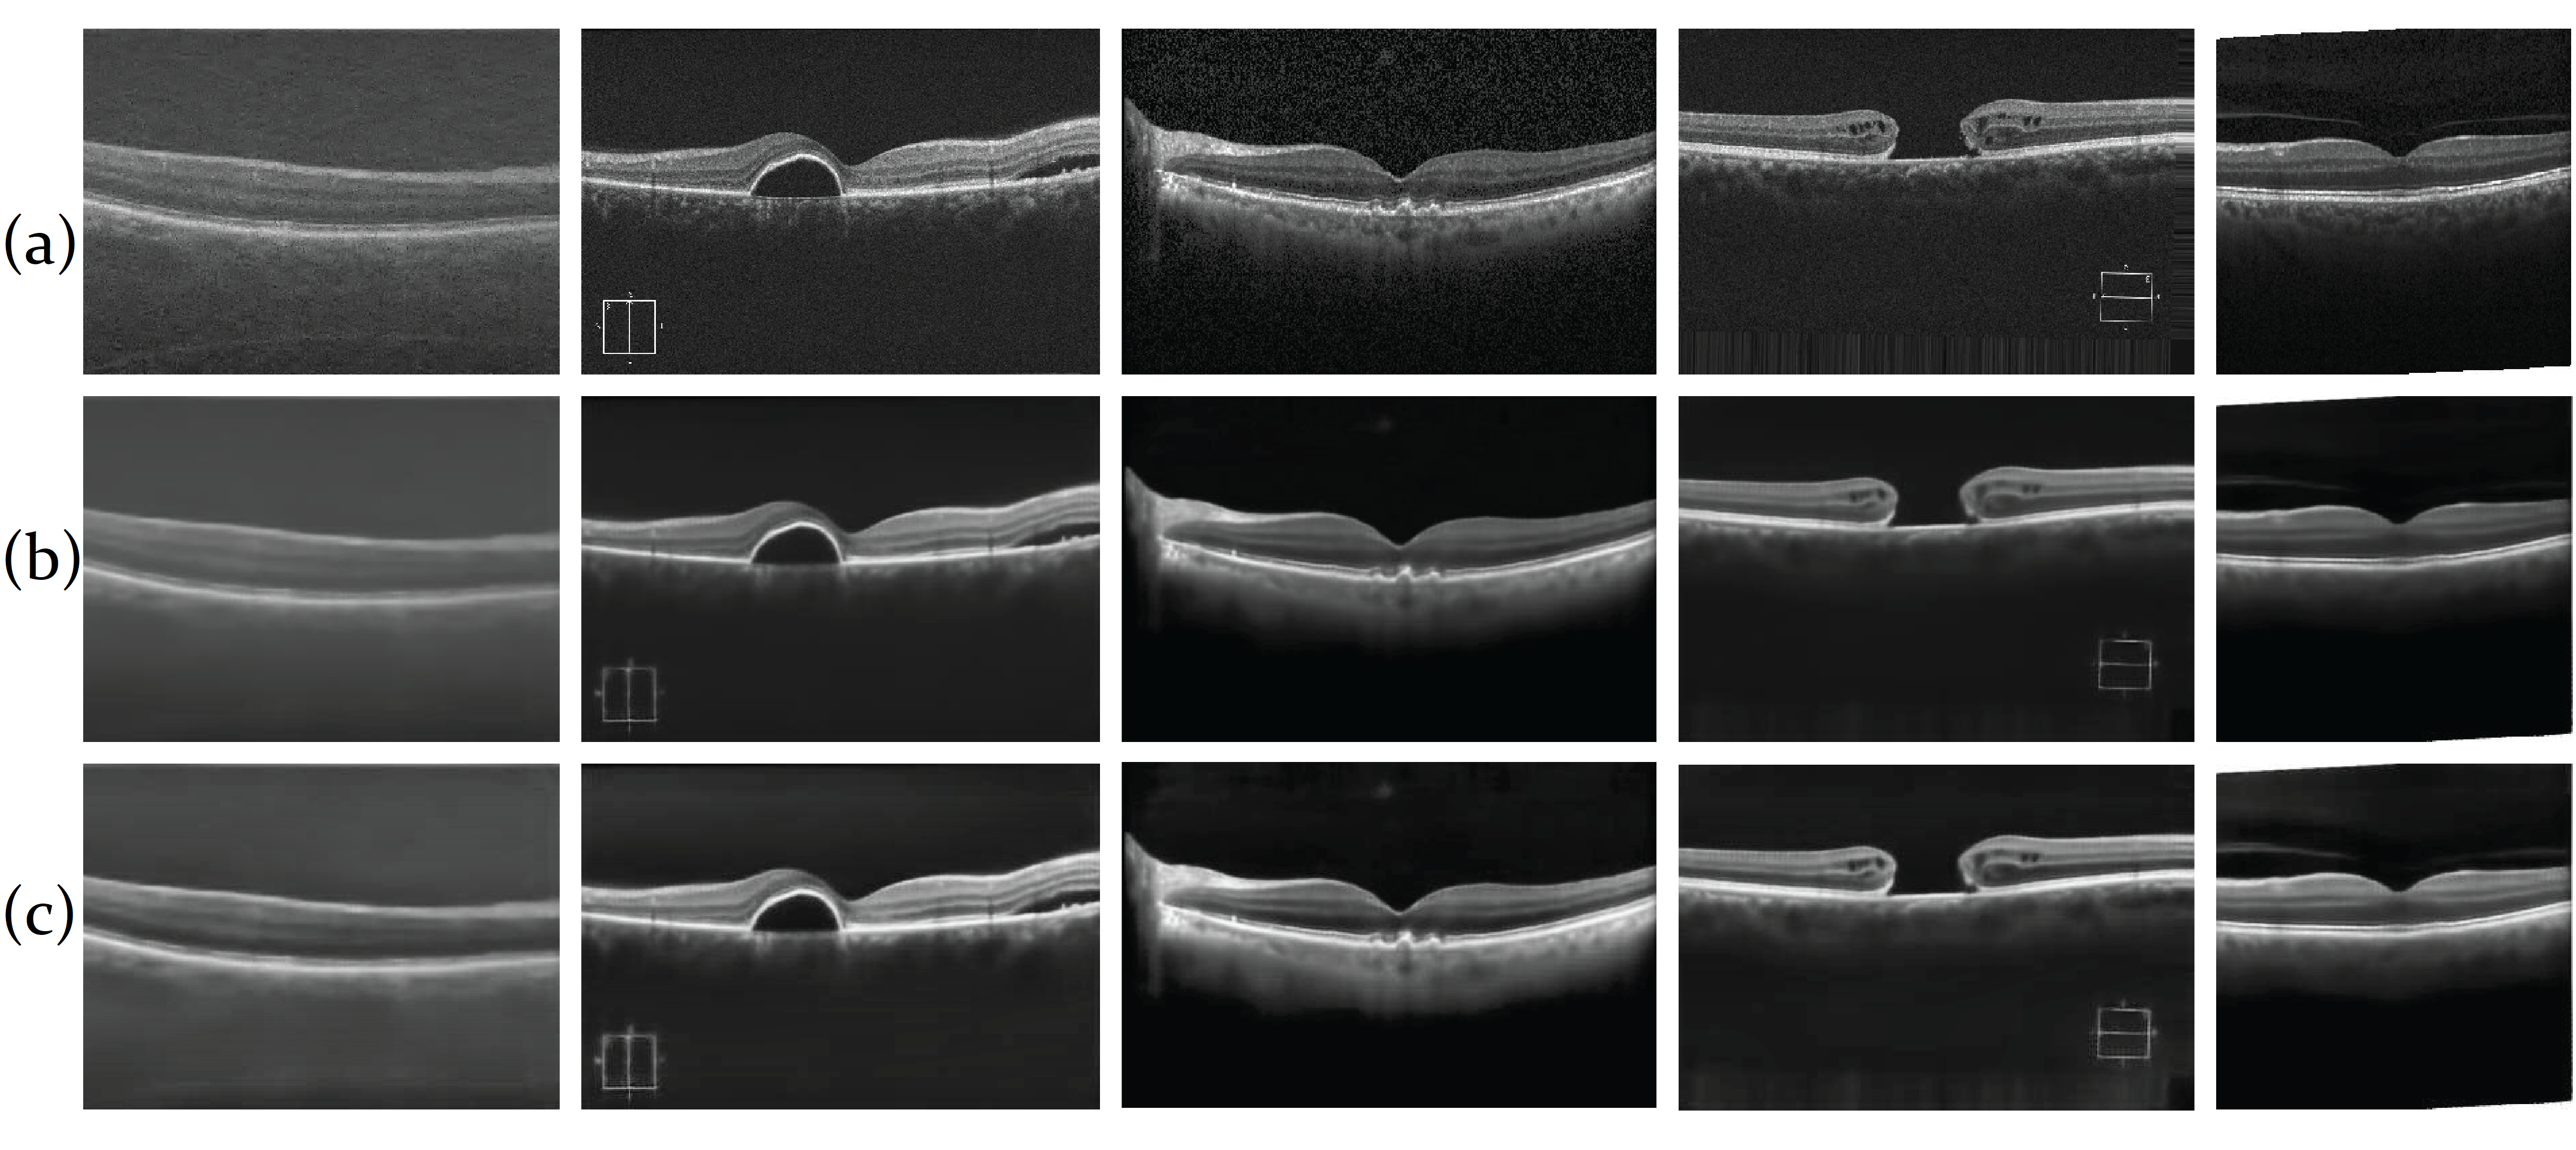
\includegraphics[width=\linewidth]{figimages/Comparison.png}
\caption{Comparison between (a) Raw images, (b) De-noised images and (c) Contrast Adjusted images} 
\label{fig: comparison}
\end{figure}

\subsection{Five-layered CNN}
\vspace{1em}
After successful training, various evaluation parameters have been set to judge the performance and validate the models. The Figure \ref{fig:trainingAcc5CNN} and \ref{fig:trainingLoss5CNN} show the plots from the training phase. 

\begin{figure}[htb]
\centering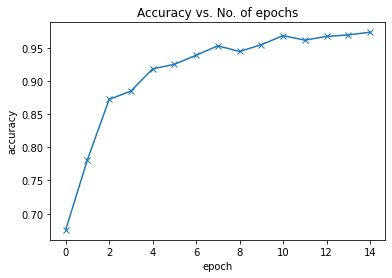
\includegraphics[width=0.75\linewidth]{figimages/acc5Layered.png}
\caption{Training Accuracy plot for Five-layered CNN} 
\label{fig:trainingAcc5CNN}
\end{figure}
\begin{figure}[htb]
\centering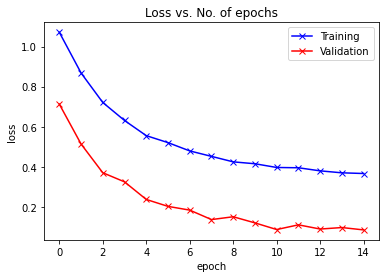
\includegraphics[width=0.75\linewidth]{figimages/loss5Layered.png}
\caption{Loss plot for Five-layered CNN} 
\label{fig:trainingLoss5CNN}
\end{figure}
\newpage

\par
The Five-layered CNN model achieves the highest validation accuracy of 97.33\% and minimum validation loss of 0.08. The F1 score calculated is 97.32. Table \ref{table: performance} shows the evaluation parameters including precision, recall, etc. The confusion matrix obtained for the same is shown in Figure \ref{fig:conf5CNN}.

\begin{table}[ht]
\centering
\caption{Performance parameters of the proposed classification models}
\renewcommand{\arraystretch}{2} 
\begin{tabular}{|c|c|c|}
\hline
\textbf{Parameter} & \textbf{Five-layered CNN} & \textbf{Bottleneck CNN} \\ \hline
Epochs & 15 & 15 \\ \hline
Learning Rate & 1 x $10^{-5}$ & 5.5 x $10^{-5}$ \\ \hline
Minimum Training Loss & 0.37 & 0.04 \\ \hline
Minimum Validation Loss & 0.08 & 0.07 \\ \hline
Maximum Validation Accuracy & 97.33\% & 97.50\% \\ \hline
Recall Accuracy (AMD) & 100\% & 100\% \\ \hline
Recall Accuracy (Normal) & 95.71\% & 99.71\% \\ \hline
Recall Accuracy (Drusen) & 94.28\% & 89.14\% \\ \hline
Recall Accuracy (CSR) & 97.14\% & 98.85\% \\ \hline
Recall Accuracy (MH) & 99.42\% & 99.71\% \\ \hline
Precision (AMD) & 99.43\% & 99.71\% \\ \hline
Precision (Normal) & 97.66\% & 96.67\% \\ \hline
Precision (Drusen) & 94.55\% & 98.42\% \\ \hline
Precision (CSR) & 94.97\% & 93.01\% \\ \hline
Precision (MH) & 100\% & 100\% \\ \hline
F1 Score & 97.32 & 97.46 \\ \hline
\end{tabular}
\label{table: performance}
\end{table}

\begin{figure}[H]
\centering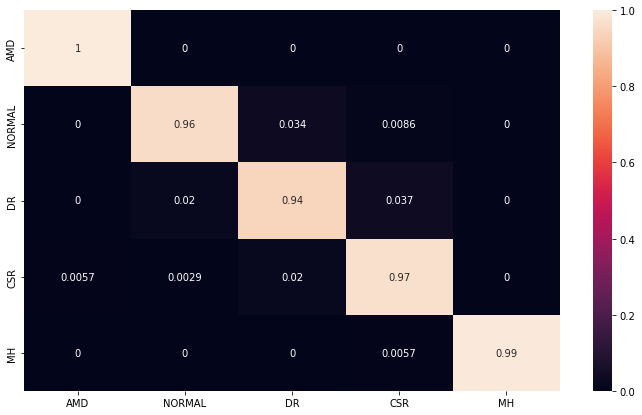
\includegraphics[width=0.75\linewidth]{figimages/confusion5Layered.png}
\caption{Confusion Matrix for Five-layered CNN} 
\label{fig:conf5CNN}
\end{figure}


\subsection{Bottleneck CNN}
\vspace{1em}
The Figure \ref{fig:trainingAccbottle} and \ref{fig:trainingLossbottle} show the plots from the training phase.

\begin{figure}[H]
\centering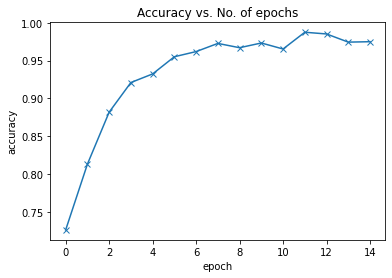
\includegraphics[width=0.75\linewidth]{figimages/accBottleneck.png}
\caption{Training Accuracy plot for Bottleneck CNN} 
\label{fig:trainingAccbottle}
\end{figure}

\begin{figure}[H]
\centering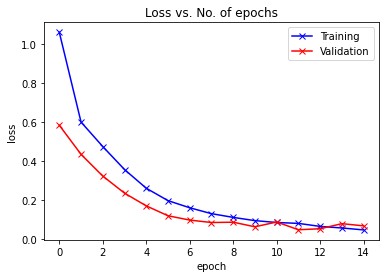
\includegraphics[width=0.75\linewidth]{figimages/lossBottleneck.png}
\caption{Loss plot for Bottleneck CNN} 
\label{fig:trainingLossbottle}
\end{figure}

The Bottleneck CNN model achieves the highest validation accuracy of 97.50\% and minimum validation loss of 0.07. The F1 score for the model is 97.46. Table \ref{table: performance} shows the evaluation parameters including precision, recall, etc. The confusion matrix obtained for the same is shown in Figure \ref{fig:confBottle}.

\begin{figure}[H]
\centering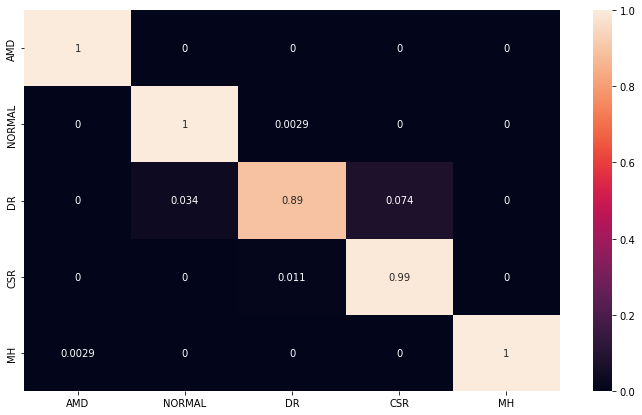
\includegraphics[width=0.75\linewidth]{figimages/confusionBottleneck.png}
\caption{Confusion Matrix for Bottleneck CNN} 
\label{fig:confBottle}
\end{figure}

\section{Discussion}
There have been different methods and algorithms used for classification of retinal diseases using OCT scans- raw, segmented, unsegmented etc. over the years. Some of the prominent research works are taken into consideration in this section.

\par
Hussain et al. \cite{Hussain2018} proposed a classification technique for OCT images of AMD and DME. The method involved image segmentation on the raw OCT scans before classification. The data was made of total 1,183 images consisting of 238 normal, 885 AMD, and 60 DME images. The method used Random Forest \cite{Breiman2001} algorithm for classification with a 95\% accuracy.

\par
Maetschke et al. \cite{Maetschke2019} devised a different approach with unsegmented raw OCT images. The technique consisted of a binary CNN classifier, classifying images of Glaucoma disease and normal eye. The data consists of 1,110 images with 263 healthy normal eye and 847 glaucoma effected images. The proposed method consists of five 3-D Convolutional layers with ReLU activation and Batch Normalization layers. The binary classifier had a 94\% accuracy.

\par
Feng et al. \cite{Li2019} devised a classification technique for DME, CNV, Drusen and normal eye classes. The data consists of a total 21,357 images. The data was classified using multi-ResNet50 ensemble. The proposed transfer learning method achieved an accuracy of 97.3\%.

\par
Tayal et. al.\cite{Tayal2022} proposed three novel CNN classifiers consisting of 5, 7 and 9 Convolutional layers respectively. The data consists of a total of 83,484 images. The best validation accuracy is achieved by 5-layered CNN model with an accuracy of 96.30\%. The images were denoised using median filters, contrast adjusted using CLAHE algorithm and fed to CNN classifier. The 4-class CNN is made of convolutional layers connected through pooling layers, followed by 3 linear layers and a 40\% dropout layer.

\par
Table \ref{table:discussion} demonstrates the efficacy comparison of existing techniques to the proposed approach. The proposed Bottleneck CNN along with denoising using Autoencoder outperforms the previous approaches by achieving an accuracy of 97.50\%.

\begin{table}[ht]
\centering
\caption{Comparison of performances of different methods with the proposed method}
\renewcommand{\arraystretch}{2} 
\begin{tabular}{|c|c|c|}
\hline
\textbf{Paper} & \textbf{Minimum Loss} & \textbf{Maximum Accuracy (\%)} \\ \hline
\cite{Li2019} & - & 97.30 \\ \hline
\cite{Tayal2022} & 0.15 & 96.30 \\ \hline
\cite{Maetschke2019} & - & 94 \\ \hline
\cite{Hussain2018} & - & 95 \\ \hline
Proposed & 0.07 & 97.50 \\ \hline
\end{tabular}
\label{table:discussion}
\end{table}


% ~
\vspace{8cm}
\begin{center}
$\qquad $ 
\end{center}
\vfill
~

% chapter 5
\chapter{Conclusion and Future Scope}
\label{chapter:conclusion} 
\noindent\rule{\linewidth}{2pt}

\section{Conclusion}
In this research work, the use of novel CNN for classifying OCT images, with a particular focus on improving accuracy through noise removal using an autoencoder has been explored. It has been observed that the noise removal  using convolutional autoencoder outperformed the existing method with  MSE value of 0.002 and PSNR value of 27.324 dB. The proposed method has been evaluated through various parameters such as precision, F1 score, and recall factor. The proposed novel CNN architecture  outperformed the previous methods with an impressive accuracy of 97.50\%. 

\section{Future Scope}
These findings have important implications for the field of medical image analysis, where accurate and efficient image classification is crucial for effective diagnosis and treatment. The results of this study demonstrate the potential of deep learning techniques for improving the accuracy and efficiency of OCT image analysis, and suggests exciting possibilities for future research in this area.
% ~
\vspace{8cm}
\begin{center}
$\qquad $ 
\end{center}
\vfill
~

\newpage
\pagestyle{plain}
\singlespacing
\chapter*{Author's Contribution} 
\noindent\rule{\linewidth}{2pt}

\begin{itemize}
    \item [{[1]}] Srivastava, A., Kumar, A. and Jaiswal A.(2023). Ocular Disease Classification using OCT Scans and Deep Learning: CNN and Autoencoders.  Expert Systems With Applications. (Communicated)
\end{itemize}

\addcontentsline{toc}{chapter}{Author's Contibution}

%\appendix
%\include{Chapters/appendix/appendix}

~
\vspace{8cm}
\begin{center}
$\qquad $ 
\end{center}
\vfill
~
\pagestyle{plain}

% \chapter*{Bibliography} 
% \noindent\rule{\linewidth}{2pt}

% \addcontentsline{toc}{chapter}{Bibliography}
% \singlespacing
% \printbibliography[heading=none]






%\addcontentsline{toc}{chapter}{List of publications}
%\include{Chapters/publications/publications}
\singlespacing
\bibliographystyle{IEEEtran}
\renewcommand{\bibname}{References}
% \noindent\rule{\linewidth}{2pt}
\addcontentsline{toc}{chapter}{References}
\bibliography{References}
% \noindent\rule{\linewidth}{2pt}

% \newpage
% \includepdf[pages={1}]{Initial_Pages/similarity.pdf}

% \newpage
% \includepdf[pages={1}]{plag_report_lib.pdf}

%$$
%--\times --\times --\times --
%$$
\end{document}
